\chapter{Electrones identificados como fotones}\label{ch:e_fake}
\chaptermark{Electrones identificados como fotones}


Como ya se mencionó anteriormente, existe un fondo que contribuye a procesos asociados a fotones, jets y energía perdida como estado final, donde un electrón del estado final es identificado como un fotón. Este puede provenir de procesos del SM, como los que producen bosones $W$ y $Z$ + jets, y $\ttbar$. El mismo es difícil de estimar a partir de simulaciones, ya que depende en gran medida de la estructura y material del detector que es muy compleja de modelar en todos sus detalles. El objetivo es entonces estimar este fondo calculando un factor de identificación errónea (\textit{Fake Factor}) en función de las variables $\eta$ y $p_{T}$ de los objetos, a partir de los datos adquiridos por el detector ATLAS durante la toma de datos de 2015 y 2016.

\section{Determinación del factor de identificación errónea}

El método para la estimación del factor de identificación errónea, hace uso de la muestra de eventos $Z\rightarrow ee$. En base a esta muestra se determinan la relación de eventos de pares electrón-positrón y los paras electrón(positrón)-fotón cuya masa invariante es compatible con la del bosón $Z$. Estos últimos pares así seleccionados provienen de eventos en los cuales un electrón (positrón) del decaimiento del $Z$ es reconstruido como un fotón. El factor de identificación espuria se puede calcular entonces como: 

\begin{equation}
F_{e\rightarrow\gamma}[\eta , p_{T}]=\frac{N^{e\gamma}[\eta , p_{T}]}{N^{ee}[\eta , p_{T}]} \label{eq:ff_ratio}
\end{equation}

\noindent
donde $N^{e\gamma}$ y $N^{ee}$ son la cantidad de pares $e\gamma$ y $ee$ respectivamente, con un cierto $\eta$ y $p_{T}$ de uno de sus objetos convenientemente seleccionados.

Los criterios para seleccionar los objetos de los pares de partículas mencionados se explican a continuación y se basan en criterios de selección que mantengan una alta pureza de la muestra, manteniendo un bajo rechazo de señal.
Los electrones  son seleccionados con $p_{T} > 25 \egev$, con un criterio de calidad tanto \textit{tight} como \textit{medium}, y punto de trabajo de aislamiento \textit{gradient loose} \cite{ATLAS-CONF-2016-024}. Para los fotones los requisitos son $p_{T} > 25 \egev$, \textit{tight} y aislados \cite{STDM-2010-08}. A ambos se les solicita que tengan un $\eta_{BE}<2.37$; que estén fuera de la región del \textit{crack} entre $1.37$ y $1.52$; que provengan del vértice primario en base a un parámetro de impacto $d_{0}$ con una significancia menor a 5, y que cumplan con la relación $|\Delta z_{0}\sin\theta|<0.5$ mm.

Además, si un electrón y un fotón son reconstruidos con $\sqrt{\Delta\phi^{2}+\Delta\eta^{2}}<0.4$, el fotón es descartado del evento. Esto reduce precisamente la probabilidad de utilizar candidatos donde un electrón es reconstruido como fotón. Para reducir la contaminación de fondo de $W (\rightarrow e\nu)$ se aplica finalmente un selección de eventos con $\met < 40 \egev$. 


A todos los pares se les solicita una masa invariante entre $75$ y $105 \egev$  estando así en la región de cercanía a la masa del $Z$ ($91.1876 \pm 0.0021 \egev$\cite{Olive:2016xmw}). En el caso de que existiese más de un par en el evento, se utiliza el que tiene la masa invariante más cercana a la del bosón $Z$ . Esto minimiza la contaminación de pares aleatorios, descartando solo unos pocos eventos donde pueda haber más de un $Z$ en estado final.


El primer paso del método consiste en crear un arreglo bidimensional en $\eta$ y $p_{T}$ de los objetos seleccionados. Para eventos positrón-electrón una entrada se realiza para cada partícula en dicho arreglo. En los casos de pares electrón-fotón un arreglo es creado por separado y solo los valores de los fotones son utilizados. 

La concepción del método proviene de la siguiente consideración. Sea $\epsilon_{i}$ la eficiencia de reconstruir un electrón, con un valor de $\eta$ y $p_{T}$ correspondientes al bin \textit{i} del arreglo, para una muestra de \textit{N} pares de electrones y positrones reales (dentro del rango de masa), se determina a $f_{ij}$ como la fracción de pares para los cuales el electrón \textit{leading} (\textit{sub-leading}) está dentro del bin \textit{i} (\textit{j}). Considerando solamente electrones-positrones provenientes del decaimiento de un bosón $Z$, el número de eventos en el bin \textit{i} del arreglo $N^{ee}[\eta , p_{T}]$ es entonces:

\begin{equation}
N_{i}^{ee} = \sum_{i}\epsilon_{i}\epsilon_{j}f_{ij}N + \sum_{j}\epsilon_{j}\epsilon_{i}f_{ji}N = \epsilon_{i}N\sum_{j}\epsilon_{j}(f_{ij}+f_{ji})
\end{equation}

De forma análoga, ahora considerando que $p_{i}$ es la proporción de electrones reconstruidos como fotones en el bin \textit{i}, la cantidad de eventos en el bin \textit{i} del arreglo $N^{e\gamma}[\eta , p_{T}]$ es:

\begin{equation}
N_{i}^{e\gamma} = \sum_{i}p_{i}\epsilon_{j}f_{ij}N + \sum_{j}p_{j}\epsilon_{i}f_{ji}N = p_{i}N\sum_{j}\epsilon_{j}(f_{ij}+f_{ji})
\end{equation}

El factor que determina la proporción de electrones reconstruidos como fotones se define finalmente como:

\begin{equation}
F_{e\rightarrow\gamma}[\eta , p_{T}]\equiv\frac{N^{e\gamma}}{N^{ee}}=\frac{p_{i}}{\epsilon_{i}}
\end{equation}

Por ende, el factor, no es la proporción de fotones mal reconstruidos, sino que es el cociente entre esa proporción y la eficiencia de reconstruir un electrón. De esta forma el fondo correspondiente a electrones identificados como fotones resulta:

\begin{equation}
N_{e\rightarrow\gamma}(\eta , p_{T} , ... ) = F_{e\rightarrow\gamma}(\eta , p_{T})\cdot N_{e}(\eta , p_{T} , ...)
\end{equation}
	
\noindent
donde $N_{e}(\eta , p_{T} , ...)$ es el número de electrones en un determinado estado final correspondiente a las distintas regiones correspondientes a la búsqueda de partículas supersimétricas mencionadas en el capítulo anterior. Estos eventos se seleccionan entonces requiriendo un electrón en lugar de un fotón en el estado final, manteniendo fijo el resto de los cortes utilizados para definir la región de estudio. 

La implementación del método se realizó en ROOT \cite{Brun:1997pa} y C++ en base a histogramas bidimensionales. Para cada evento que contiene un par electrón-positrón, en un histograma con bines de $\eta$ y $p_{T}$ ($N^{ee}[\eta , p_{T}]$), se suma una entrada en el bin correspondiente al $\eta$ y $p_{T}$ de cada uno de los electrones. En el caso de que el evento tenga un par electrón-fotón, en otro histograma ($N^{e\gamma}[\eta , p_{T}]$), se suma una entrada en el bin correspondiente al $\eta$ y $p_{T}$ del fotón. Un esquema de este procedimiento se observa en la Figura \ref{grid}. El correspondiente factor se obtiene entonces como en la ecuación \ref{eq:ff_ratio}.

\begin{figure}
\centering
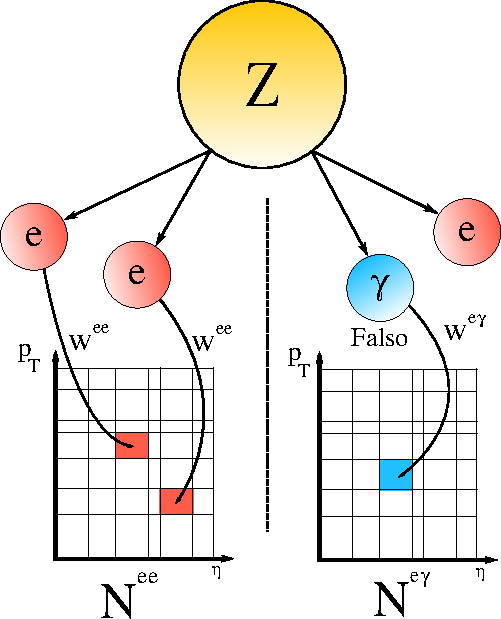
\includegraphics[width=0.45\textwidth]{grid.pdf}
\caption{Procedimiento de llenado de los histogramas $N^{ee}$ y $N^{e\gamma}$ para los pares $ee$ y $e\gamma$.}
\label{grid}
\end{figure}

La muestra de eventos $ee$ y $e\gamma$ colectada no es una muestra pura de $Z$, ya que puede incluir un fondo no resonante en los eventos generados por una combinación aleatoria de objetos o también de eventos de otros procesos electrodébiles, donde los electrones son correctamente reconstruidos o con alguno de los objetos reconstruido erróneamente. Para tener en cuenta la relación entre entradas correspondientes a la señal y las correspondientes al fondo, cada entrada en los histogramas es pesada con un peso representativo de esta relación entre señal y fondo.

% Dado que los pares de objetos utilizados para el cálculo, tienen un probabilidad de no provenir del decaimiento del bosón $Z$, sino de otros procesos no resonantes de fondo, la relación entre señal y fondo tiene en cuenta en el cálculo del factor buscado.
% Para tener en cuenta la relación entre entradas correspondientes a la señal y las correspondientes al fondo, cada entrada en los histogramas es pesada con un peso representativo de esta relación.


\section{Clasificación de eventos}

La relación entre señal y fondo de los eventos correspondientes a la masa del $Z$ se obtiene clasificando a los pares según el tipo ($ee/e\gamma$) y según la región donde se reconstruyeron los objetos \textit{endcap}-\textit{endcap} ($EE$), \textit{barrel}-\textit{endcap} ($BE$) y \textit{barrel}-\textit{barrel} ($BB$). Esto último se debe a que los factores de identificación erróneas dependen de la región del detector donde fueron reconstruidos dados los distinta morfología y tipo de detectores utilizados en cada una ellas. Para cada una de las tres regiones se calcula entonces la masa invariante de los pares, se realiza el correspondiente ajuste para determinar la contribución de señal (S) y fondo (B) y finalmente el peso resulta de la relación:

\begin{equation}
w=\frac{S}{S+B}
\label{eq:peso}
\end{equation}

Los datos utilizados para el presente análisis corresponden a los colectados durante los años 2015 y 2016 del Run 2 del LHC, en base a la denominada derivación EGAM1 (ver Sección \ref{sec:comp_model}) y sin ningún requisito adicional o particular de \textit{triggers}.

Los electrones utilizados para estimar la contaminación de fotones de señal \textit{tight}, pueden pasar tanto requerimientos  \textit{medium} como \textit{tight}. En ambos casos se encuentra una buena relación señal y fondo, siendo naturalmente el caso de selección \textit{tight} la de mayor pureza a costa de una menor estadística de la muestra. Ambas selecciones se estudian en el presente trabajo como se discute en las siguientes secciones.

Para los ajustes de la masas invariantes se utiliza como modelo de señal una \textit{double-sided Crystal-ball} (DSCB) \cite{Das:2016stf}. La misma consiste en una distribución Gaussiana cuyas ramas son reemplazadas por exponenciales. De esta forma se tiene en cuenta efectos gaussianos de resolución en la reconstrucción de los objetos y colas exponenciales que incluyen los efectos de emisión de fotones de bremsstrahlung por parte de los electrones (y sus respectivas técnicas de recuperación \cite{Kartvelishvili:2007zz}). Para el fondo se utiliza como función genérica un polinomio de grado 2. Los resultados de los ajustes obtenidos para cada clasificación de los pares se pueden observar en las Figuras \ref{fits_invmass_medium} y \ref{fits_invmass_tight}. En base a los resultados de estos ajustes se determina la contribución de señal y background en cada región, determinando así los correspondientes pesos (Ecuación \ref{eq:peso}) como se muestra en la Tabla \ref{ta:weights}.

\begin{table}[h]
\centering
\caption{Relación entre señal y fondo (Ecuación \ref{eq:peso}) obtenida para los distintos pares ($ee/e\gamma$) en cada región (EE, BE, BB), para electrones \textit{medium} y \textit{tight}. Las incertezas mostradas son estadísticas.}
\begin{tabular}{ c c c | c c }

	\hline
	\hline

	\multirow{2}{*}{Región} & \multicolumn{2}{c |}{\textit{medium e}} & \multicolumn{2}{c}{\textit{tight e}} \\

	\cline{2-5}

	 & $ee$ & $e\gamma$ & $ee$ & $e\gamma$ \\

	\hline

	EE & 0.915(2) & 0.810(7)  & 0.928(2) & 0.817(7) \\

	BE & 0.937(1) & 0.800(4)  & 0.934(1) & 0.812(5) \\

	BB & 0.9175(7) & 0.722(4)  & 0.9155(8) & 0.734(4) \\

	\hline
	\hline
\end{tabular}
\label{ta:weights}
\end{table}



\section{Incertezas sistemáticas}

% Las principales fuentes de incertezas sistemáticas del método para el cálculo de los factores que determina la contaminación de fondo en las distintas regiones, proviene de las definiciones de las funciones y rangos de ajustes de los fits, así como de las ventanas de aceptación de pares.  Para estimar los posibles incertezas se varió el rango nominal de la masa de $[75-105]\egev$ a los rangos de $[70-110]\egev$ y a $[80-100]\egev$. Como caso extremo en la definición y criterios de ajuste, se determinaron los factores imponiendo los pesos $w=1$ eliminando así la sustracción de fondo en su cálculo. Los resultados de estos estudios se muestran en la Tabla \label{ta:fftable} donde se observa que la incerteza dominante proviene en base al criterio adoptado es la de tomar $w=1$ siendo esta del orden del $20 \%$ dominando sobre todo otra contribución.

Las principales fuentes de incertezas sistemáticas del método para el cálculo de los factores que determina la contaminación de fondo en las distintas regiones, proviene tanto de los ajustes a la masa invariante como de los criterios de aceptación de los pares.  

Para estimar los posibles incertezas se varió el rango nominal de la masa de $[75-105]\egev$ a los rangos de $[70-110]\egev$ y a $[80-100]\egev$. Como caso extremo en la definición y criterios de ajuste, se determinaron los factores imponiendo los pesos $w=1$ eliminando así la sustracción de fondo en su cálculo. 

Los resultados de estos estudios para electrones \textit{medium} y \textit{tight} se muestran en las Tablas \ref{ta:fftable_medium} y \ref{ta:fftable_tight}, donde se observa que la incerteza dominante proviene de tomar $w=1$ siendo esta del orden del $20 \%$ dominando sobre todo otra contribución.

% \begin{table}
% \centering
% \begin{threeparttable}
% \caption{Incertezas sistemáticas de los factores en bines de $\eta$ y $p_{T}$. Se puede observar que el sistemático $w=1$ es el que predomina.}
% \begin{tabular}{ l l c c c }

% 	\hline
% 	\hline

% 	$|\eta|$ & $p_{T}$[GeV] & $w=1$ & Rango & Total \\
% 	\hline

% 	0 - 0.6 	& 75 - 90 	& 0.0155 & 0.0004 & 0.004 \\

% 	0 - 0.6 	& 90 - 145 	& 0.0141 & 0.0004 & 0.004 \\

% 	0 - 0.6 	& 145 - 300 & 0.0116 & 0.0008 & 0.002 \\

% 	\hline

% 	0.6 - 1.37 	& 75 - 90 	& 0.0173 & 0.0004 & 0.004 \\

% 	0.6 - 1.37 	& 90 - 145 	& 0.0161 & 0.0004 & 0.004 \\

% 	0.6 - 1.37 	& 145 - 300 & 0.0121 & 0.0008 & 0.003 \\

% 	\hline

% 	1.52 - 1.82 & 75 - 90 	& 0.036  & 0.001 & 0.00 \\

% 	1.52 - 1.82 & 90 - 145 	& 0.033  & 0.001 & 0.004 \\

% 	1.52 - 1.82 & 145 - 300 & 0.022  & 0.002 & 0.003 \\

% 	\hline

% 	1.82 - 2.37 & 75 - 90 	& 0.046		& 0.001 & 0.007 \\

% 	1.82 - 2.37 & 90 - 145	& 0.039		& 0.001 & 0.006 \\

% 	1.82 - 2.37 & 145 - 300 & 0.041		& 0.003 & 0.006 \\

% 	\hline
% \end{tabular}
% \label{ta:syst}
% \end{threeparttable}
% \end{table}

% Lo mismo se hizo con el rango del fit que se varió de su rango nominal $[70-110]\egev$, a $[65-115]\egev$ y a $[75-105]\egev$. 

% Otro sistemático surgió de la utilización de una función diferente para modelar el fondo, en este caso se usó un polinomio de grado 3. Como caso extremo en la definición y criterios de ajuste, se determinaron los factores imponiendo los pesos $w=1$ eliminando así la sustracción de fondo en su cálculo. 

%Se consideran distintas fuentes de incertezas sistemáticas. Una de ellas proveniente de la variación tanto del rango del fit, como del rango de masa de aceptación de los pares. El rango nominal del fit es $[70-110]\egev$ y se varía a $[65-115]\egev$ y a $[75-105]\egev$. El rango nominal de la masa es $[75-105]\egev$ y se varía a $[70-110]\egev$ y a $[80-100]\egev$. Se tuvo en cuenta también como fuente de sistemático, la variación en los valores de los factores al utilizar otra función para el ajuste del fondo, utilizándose un polinomio de grado 3 y un polinomio de Bernstein de grado 4.



\begin{figure}

	\begin{subfigure}{0.5\textwidth}
		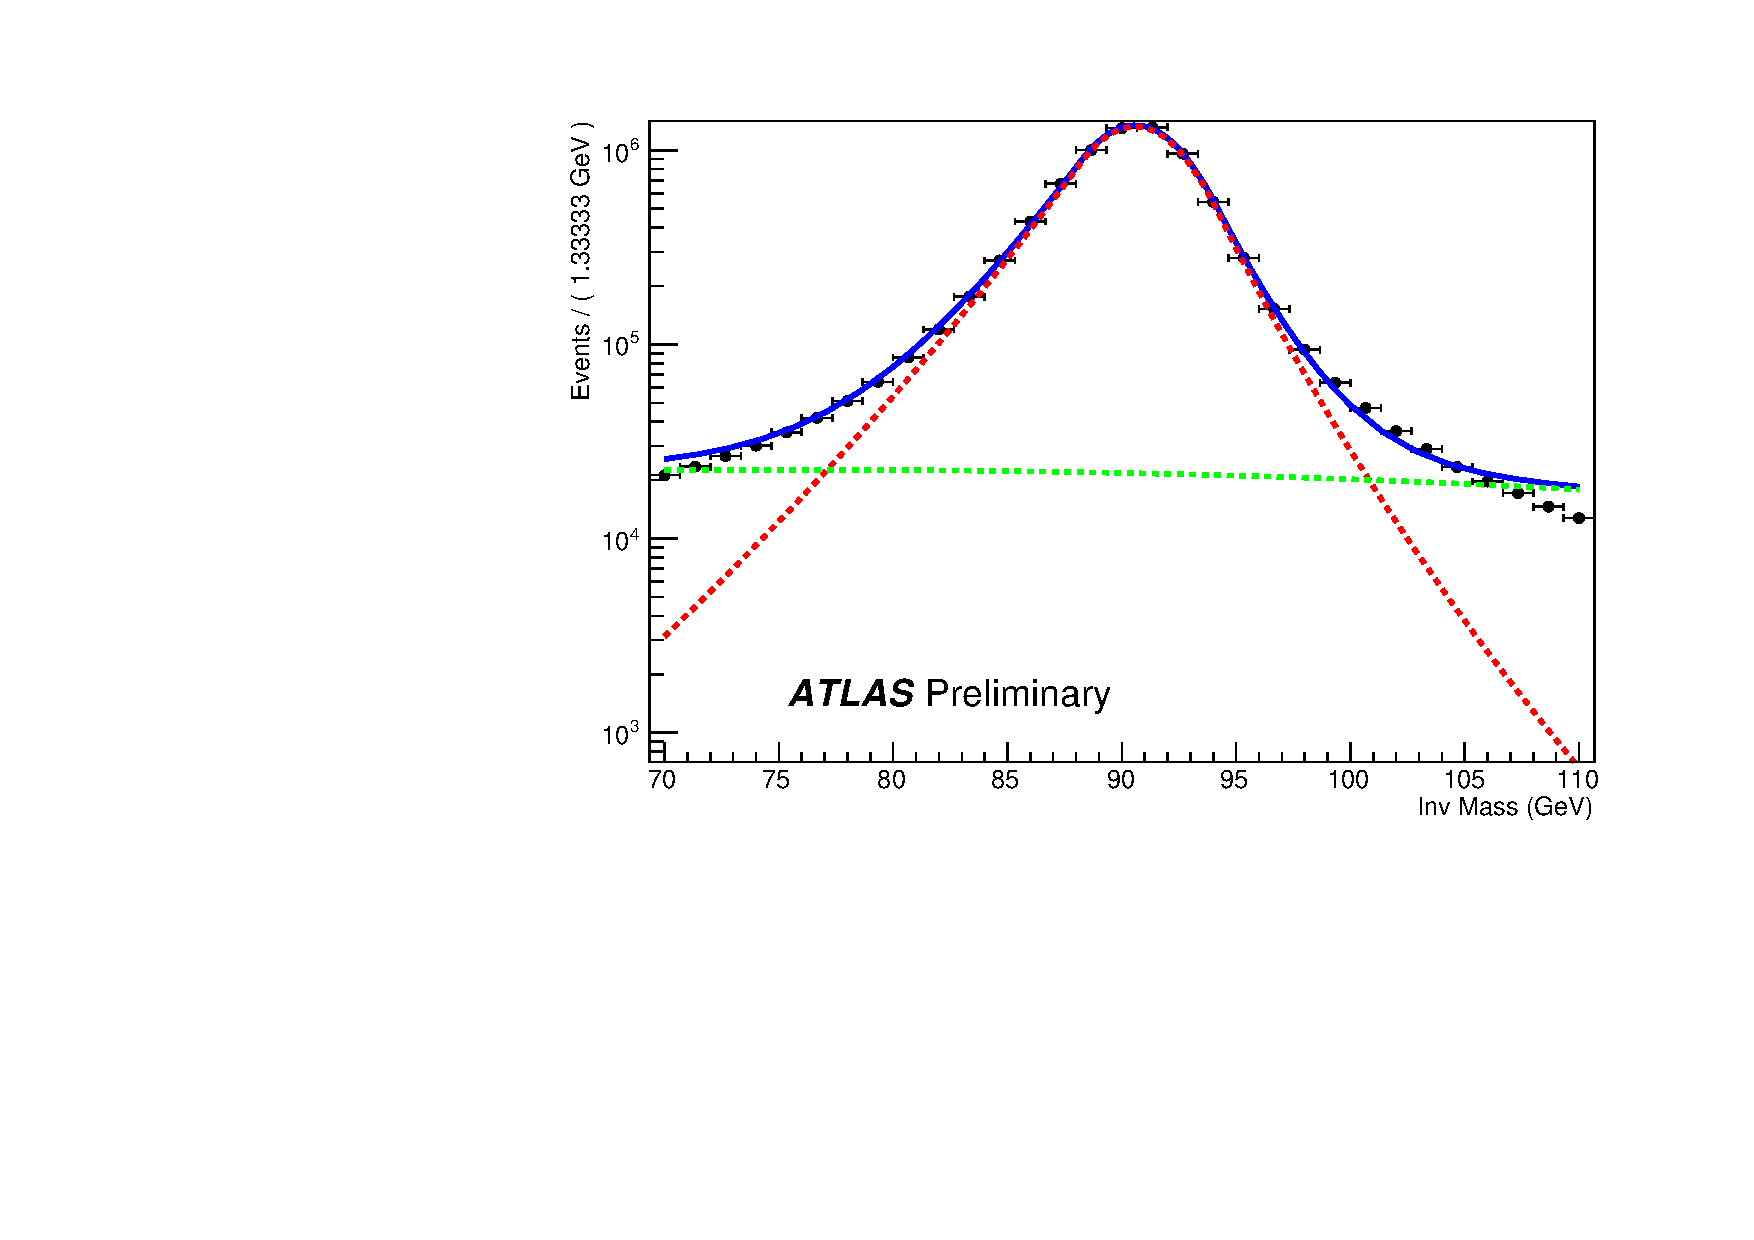
\includegraphics[scale=0.40]{d15_16_egam1_m_lmet_fit_h_m_ee_BB.pdf} 
		\caption{Región BB}
	\end{subfigure}
	~
	\begin{subfigure}{0.5\textwidth}
		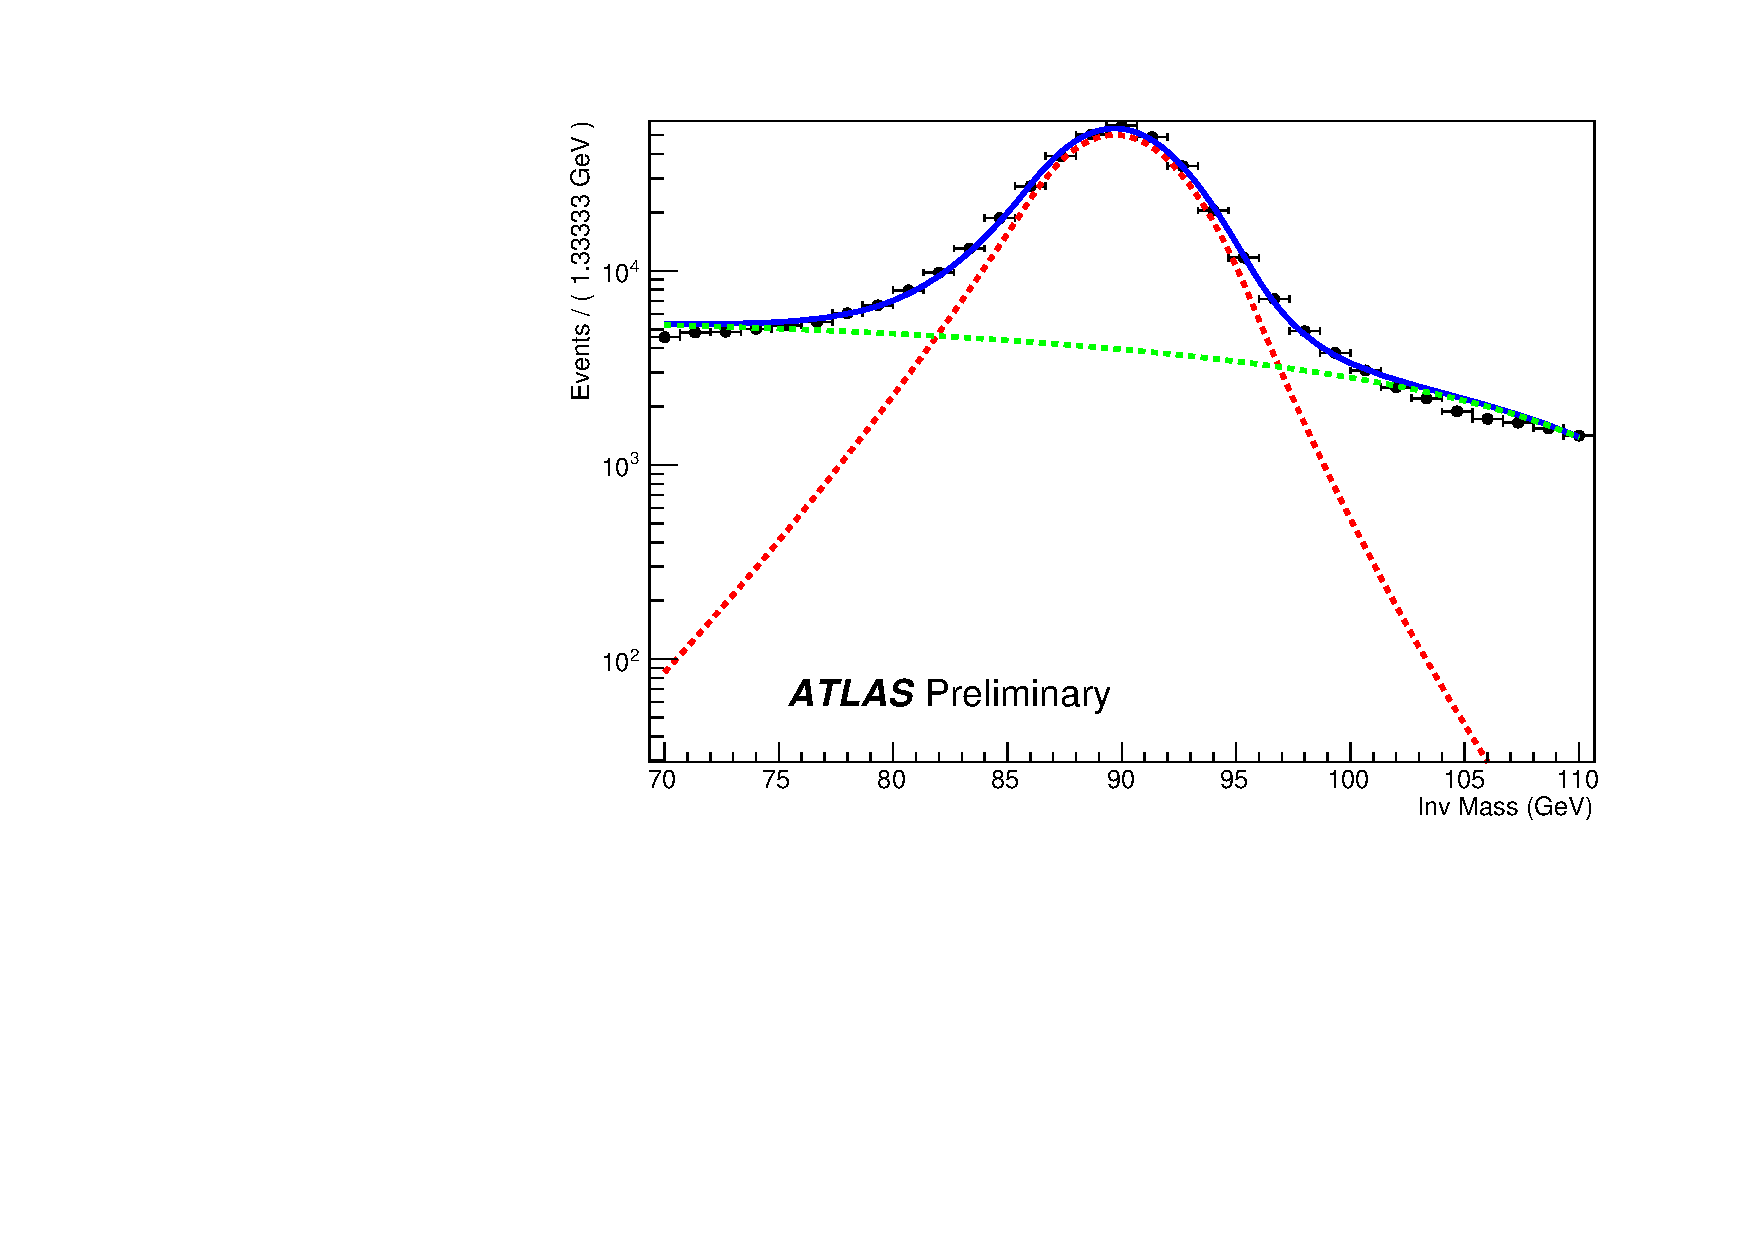
\includegraphics[scale=0.40]{d15_16_egam1_m_lmet_fit_h_m_eg_BB.pdf}
		\caption{Región BB}
	\end{subfigure}
	~
	\begin{subfigure}{0.5\textwidth}
		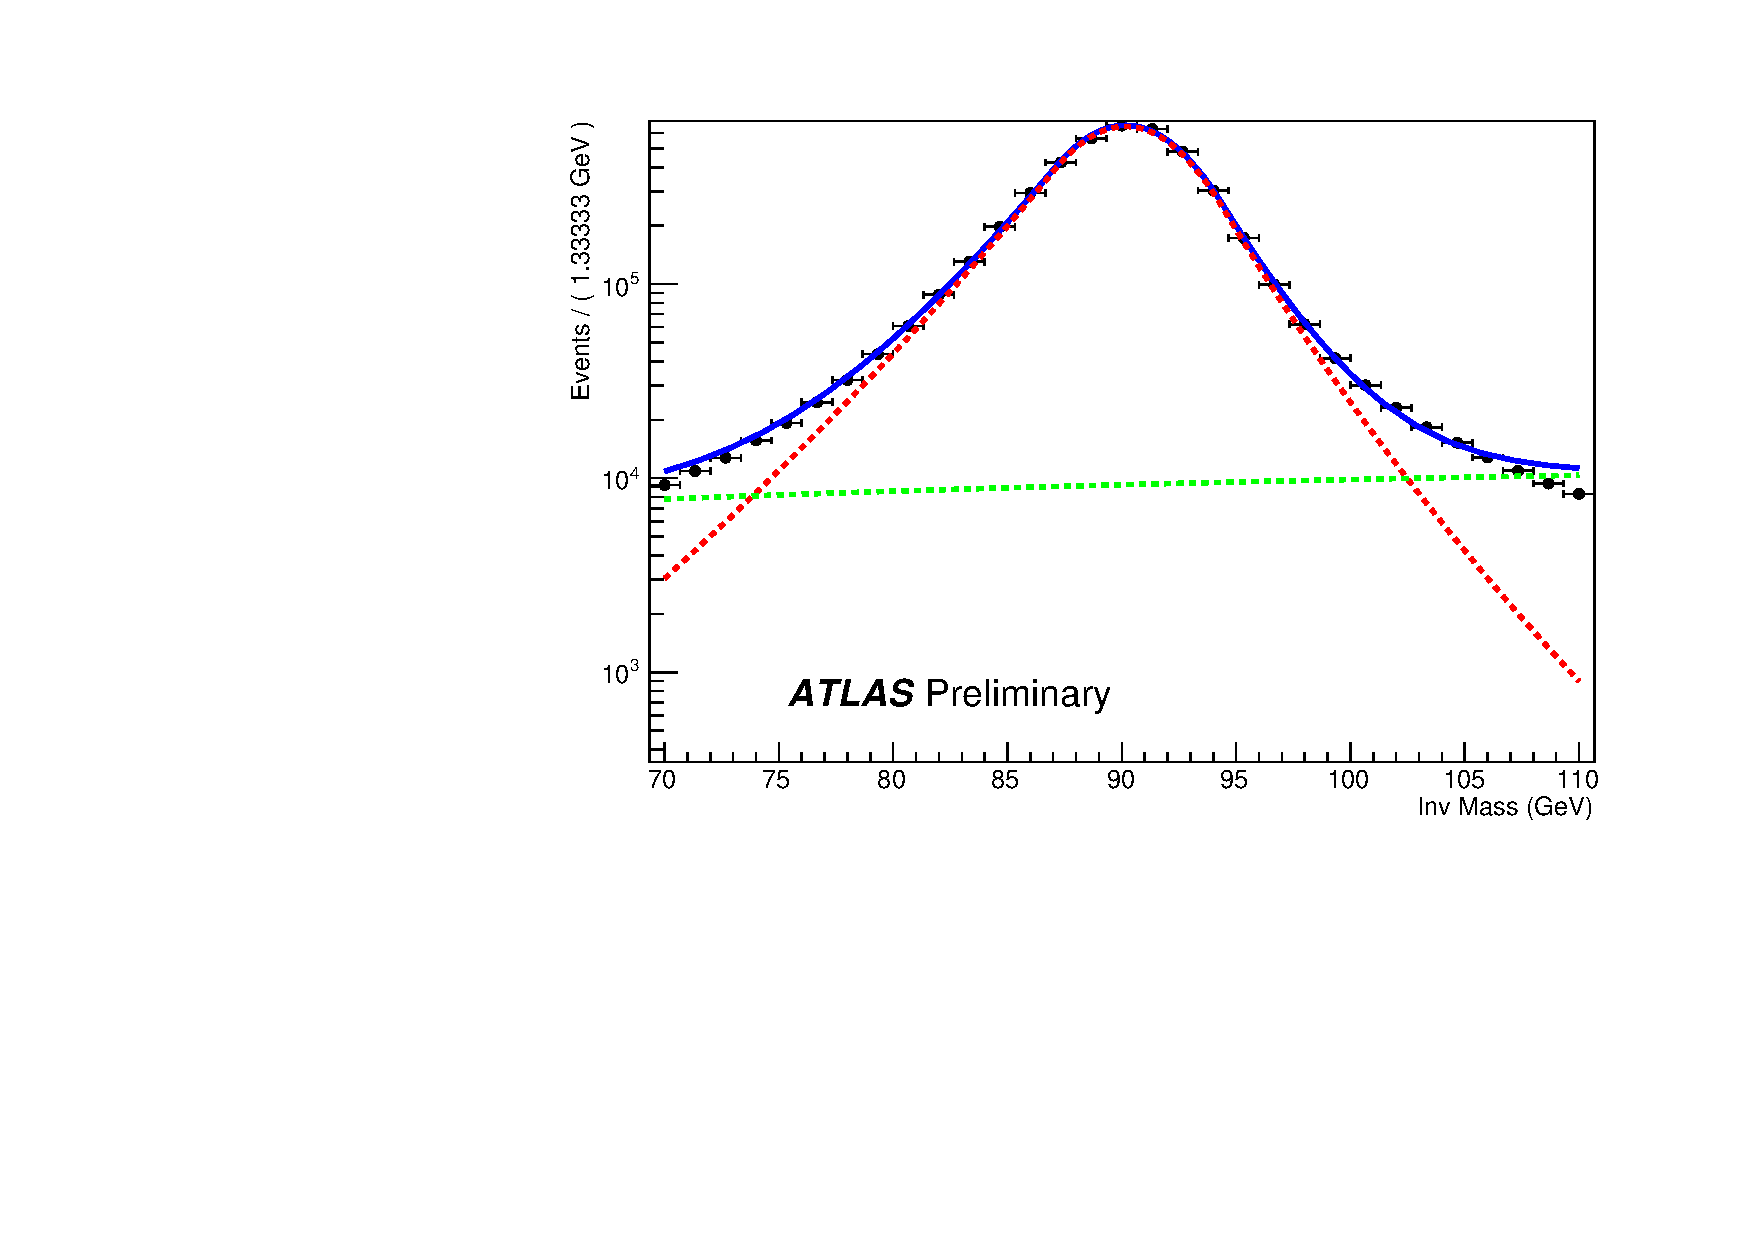
\includegraphics[scale=0.40]{d15_16_egam1_m_lmet_fit_h_m_ee_BE.pdf} 
		\caption{Región BE}
	\end{subfigure}
	~
	\begin{subfigure}{0.5\textwidth}
		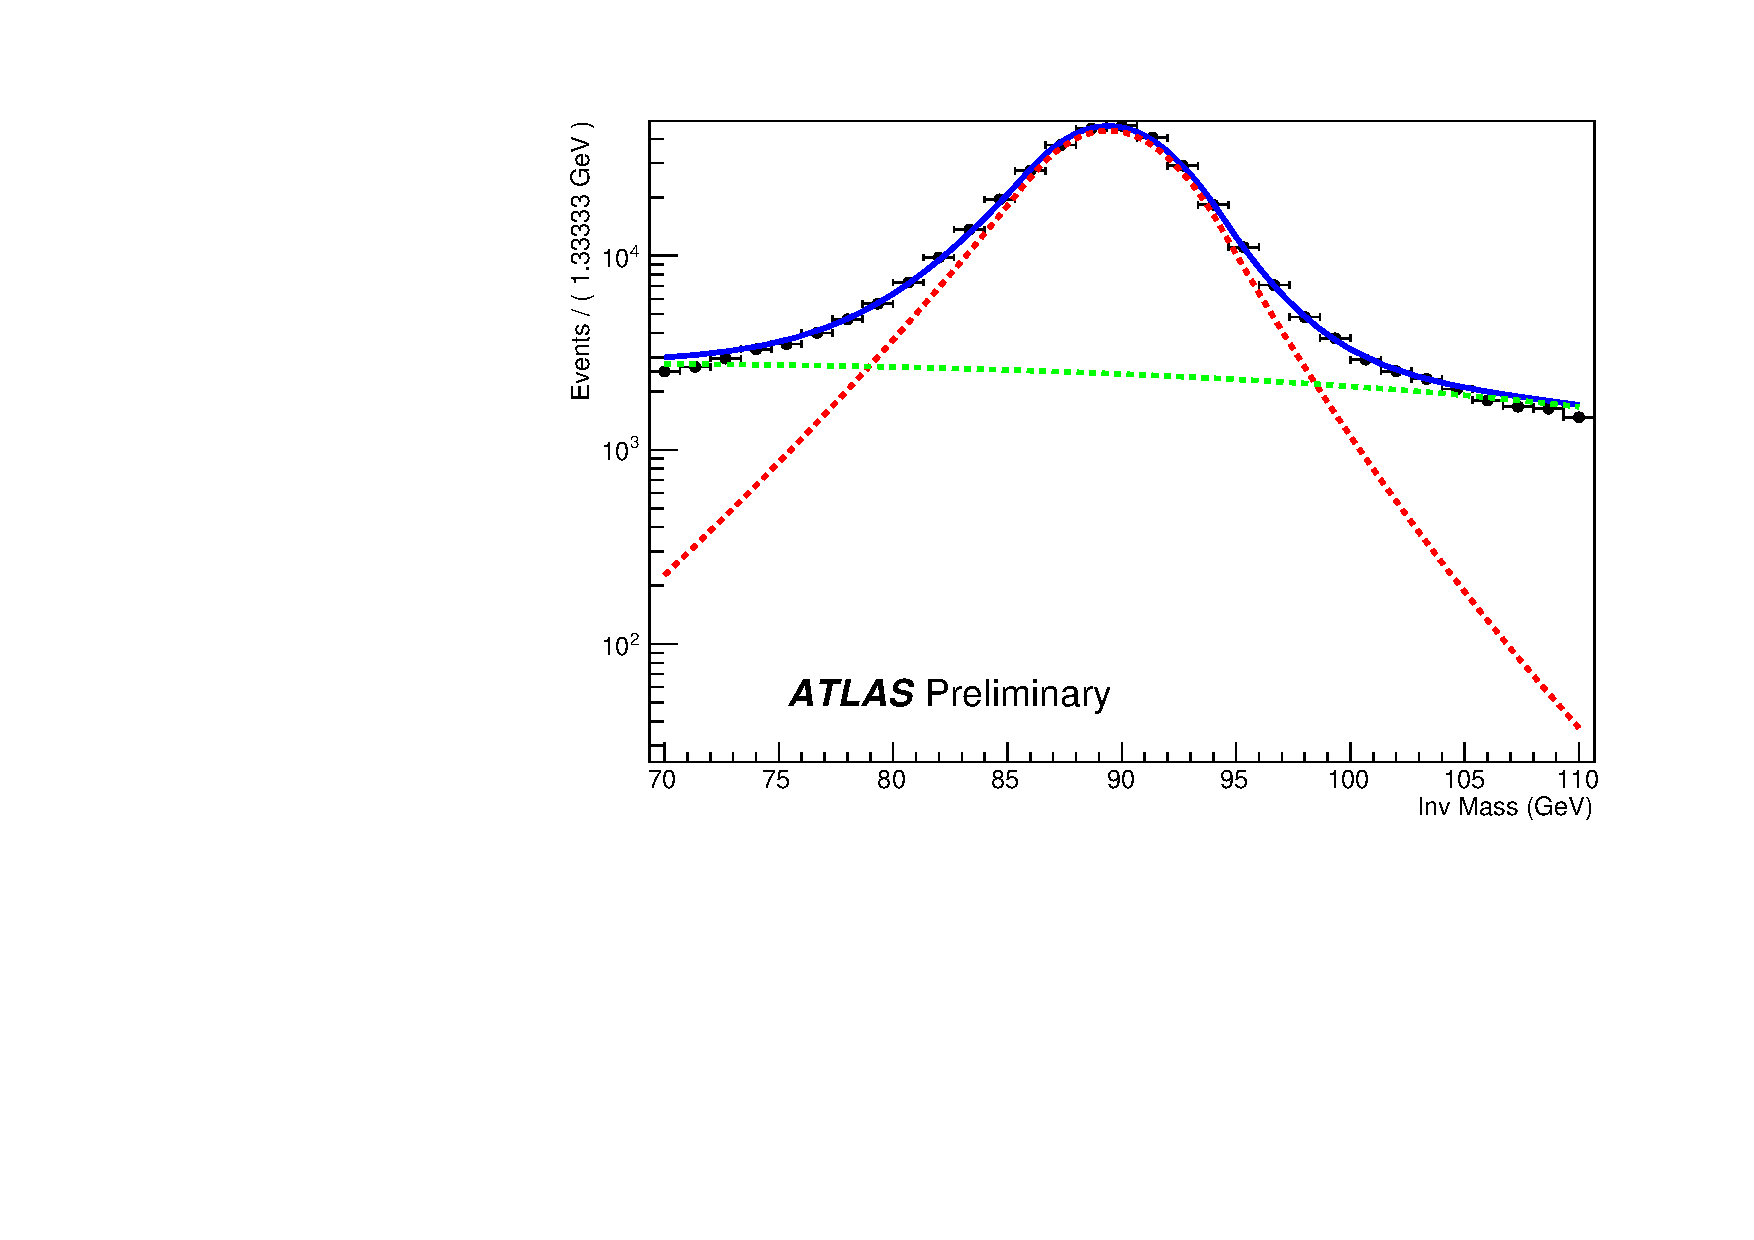
\includegraphics[scale=0.40]{d15_16_egam1_m_lmet_fit_h_m_eg_BE.pdf}
		\caption{Región BE}
	\end{subfigure}
	~
	\begin{subfigure}{0.5\textwidth}
		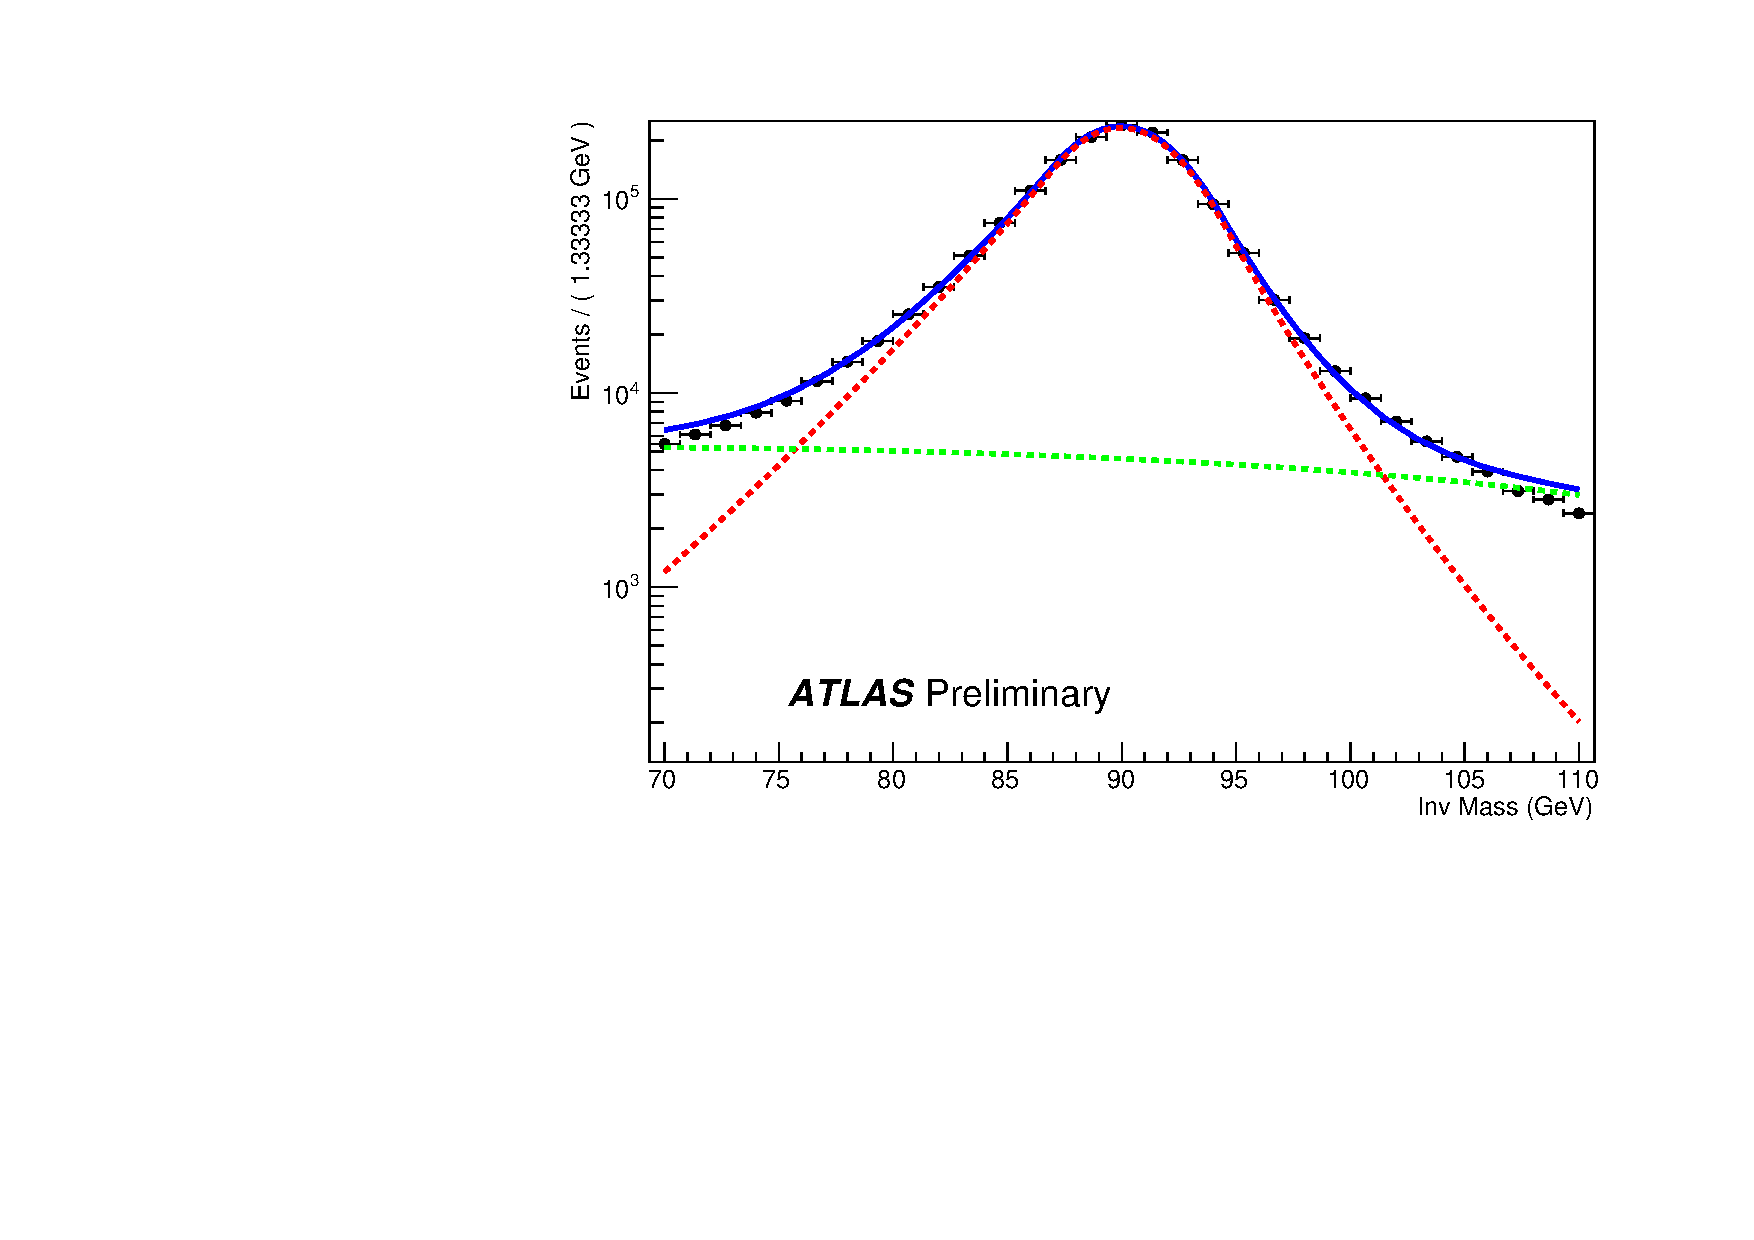
\includegraphics[scale=0.40]{d15_16_egam1_m_lmet_fit_h_m_ee_EE.pdf} 
		\caption{Región EE}
	\end{subfigure}
	~
	\begin{subfigure}{0.5\textwidth}
		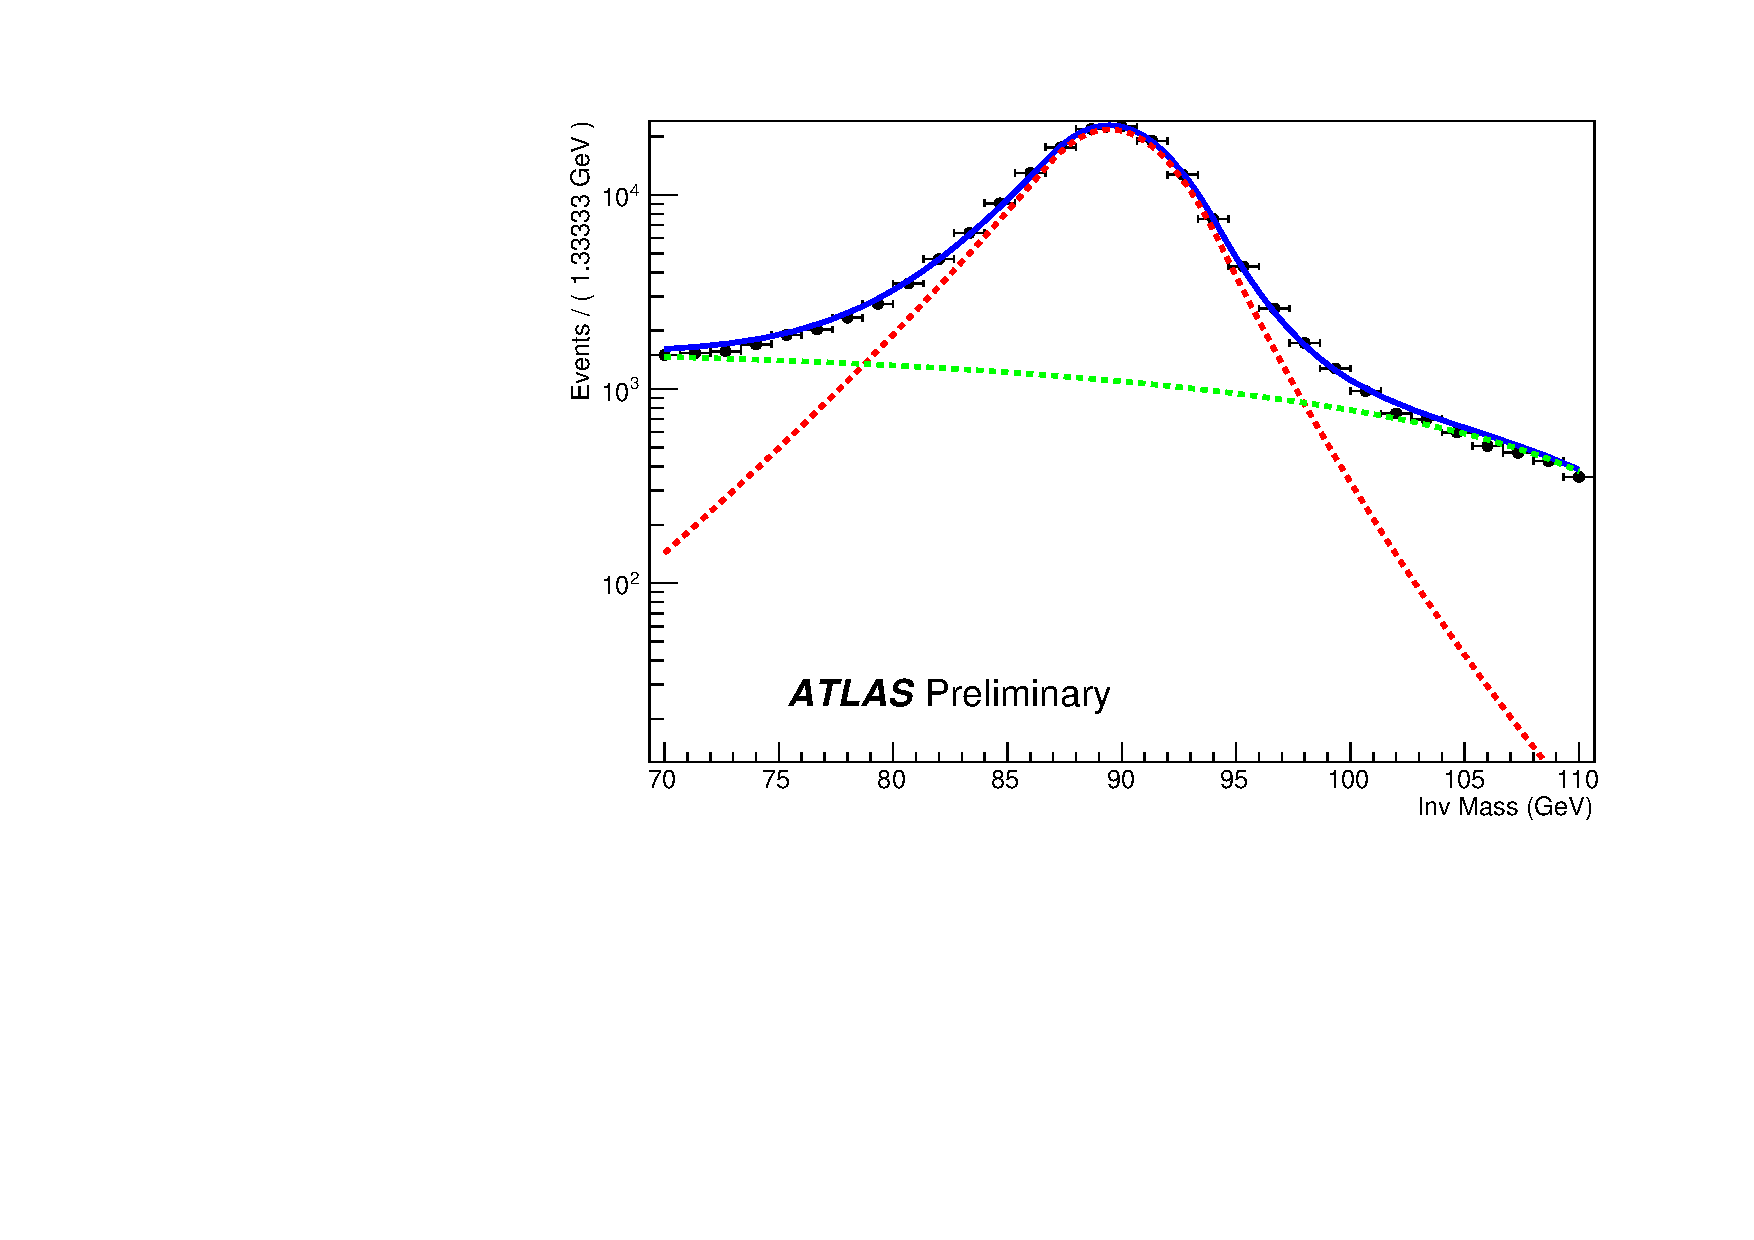
\includegraphics[scale=0.40]{d15_16_egam1_m_lmet_fit_h_m_eg_EE.pdf}
		\caption{Región EE}
	\end{subfigure}

	\caption{Ajuste de la masa invariante de los pares $ee$ (izquierda) y $e\gamma$ (derecha), para cada región de reconstrucción y para electrones \textit{medium}. La curva roja corresponde a la DSCB, la verde al polinomio de grado 2 y la azul a la combinación resultante de ambas.}
\label{fits_invmass_medium}
\end{figure}

\begin{figure}

	\begin{subfigure}{0.5\textwidth}
		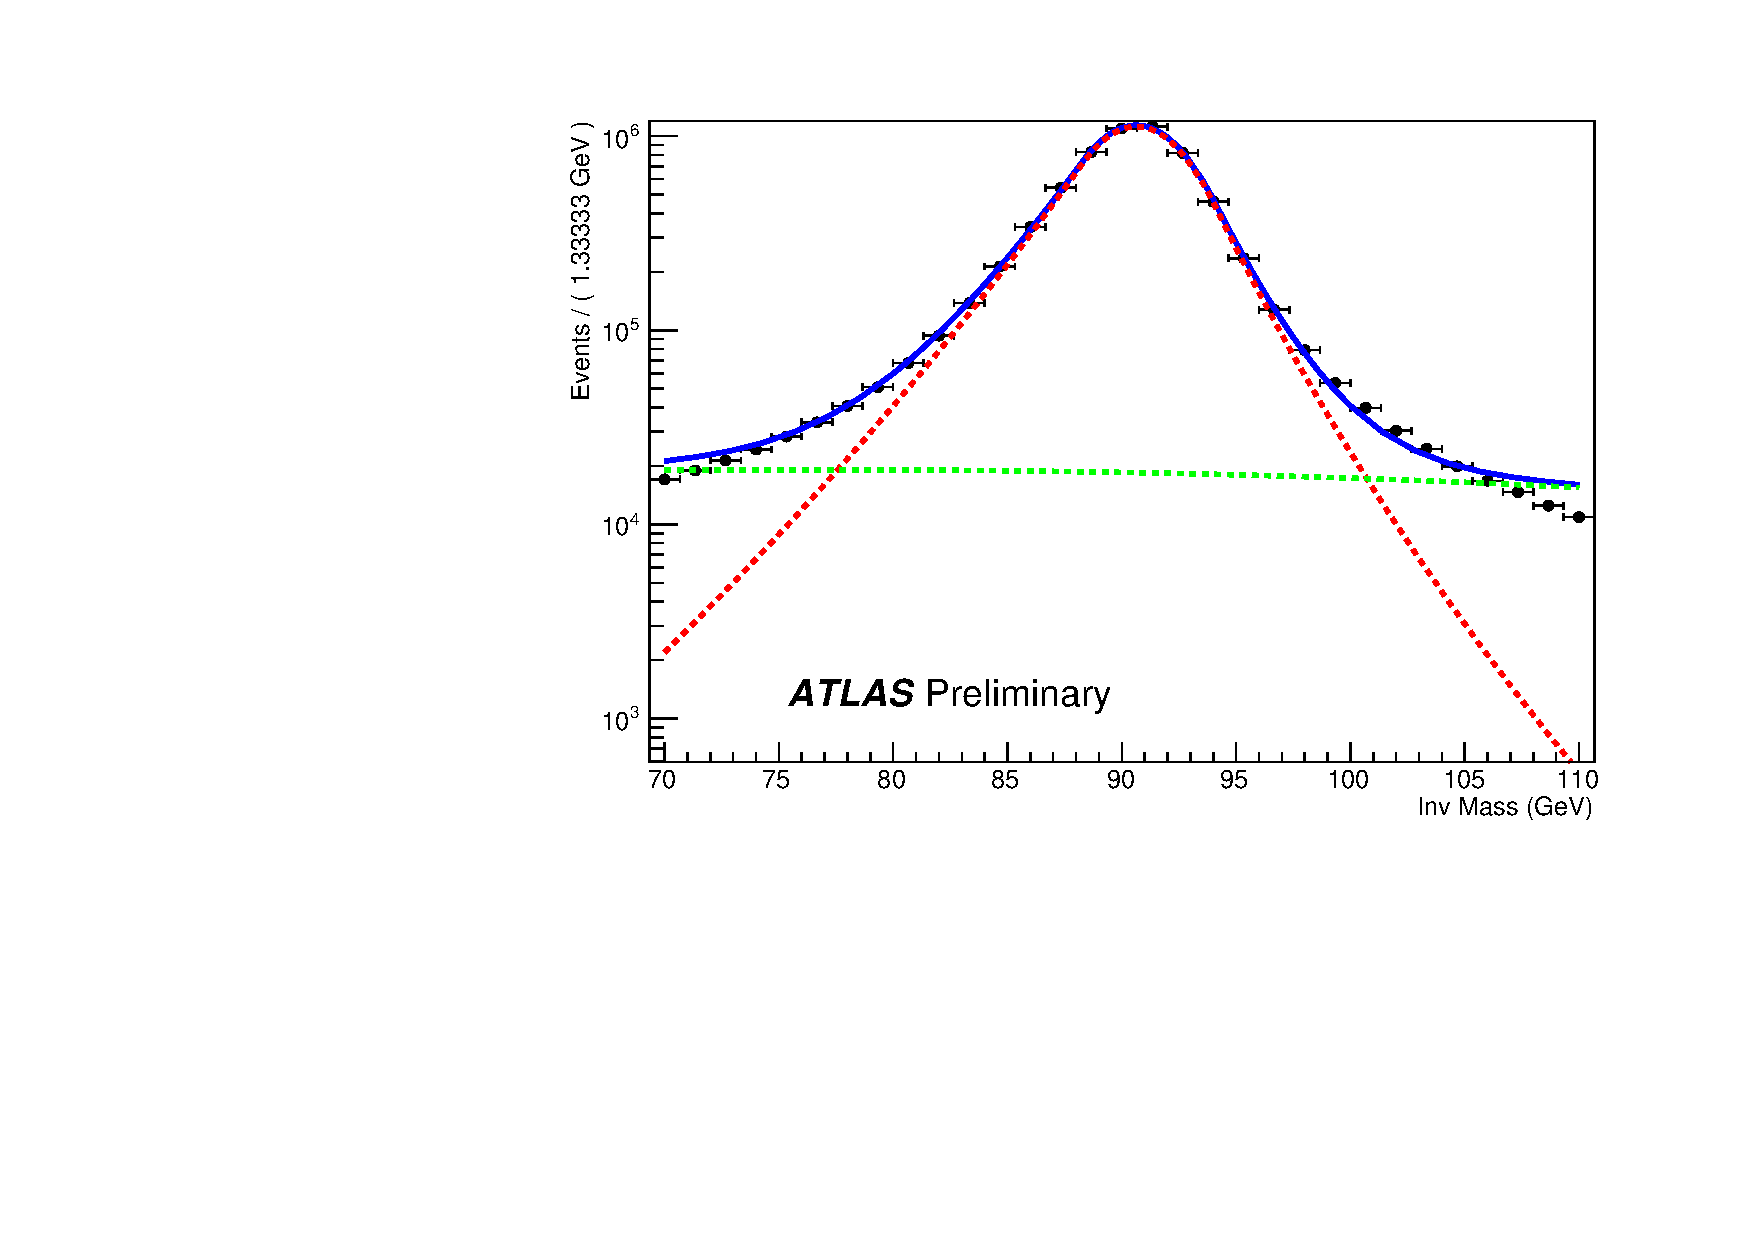
\includegraphics[scale=0.40]{d15_16_egam1_t_lmet_fit_h_m_ee_BB.pdf} 
		\caption{Región BB}
	\end{subfigure}
	~
	\begin{subfigure}{0.5\textwidth}
		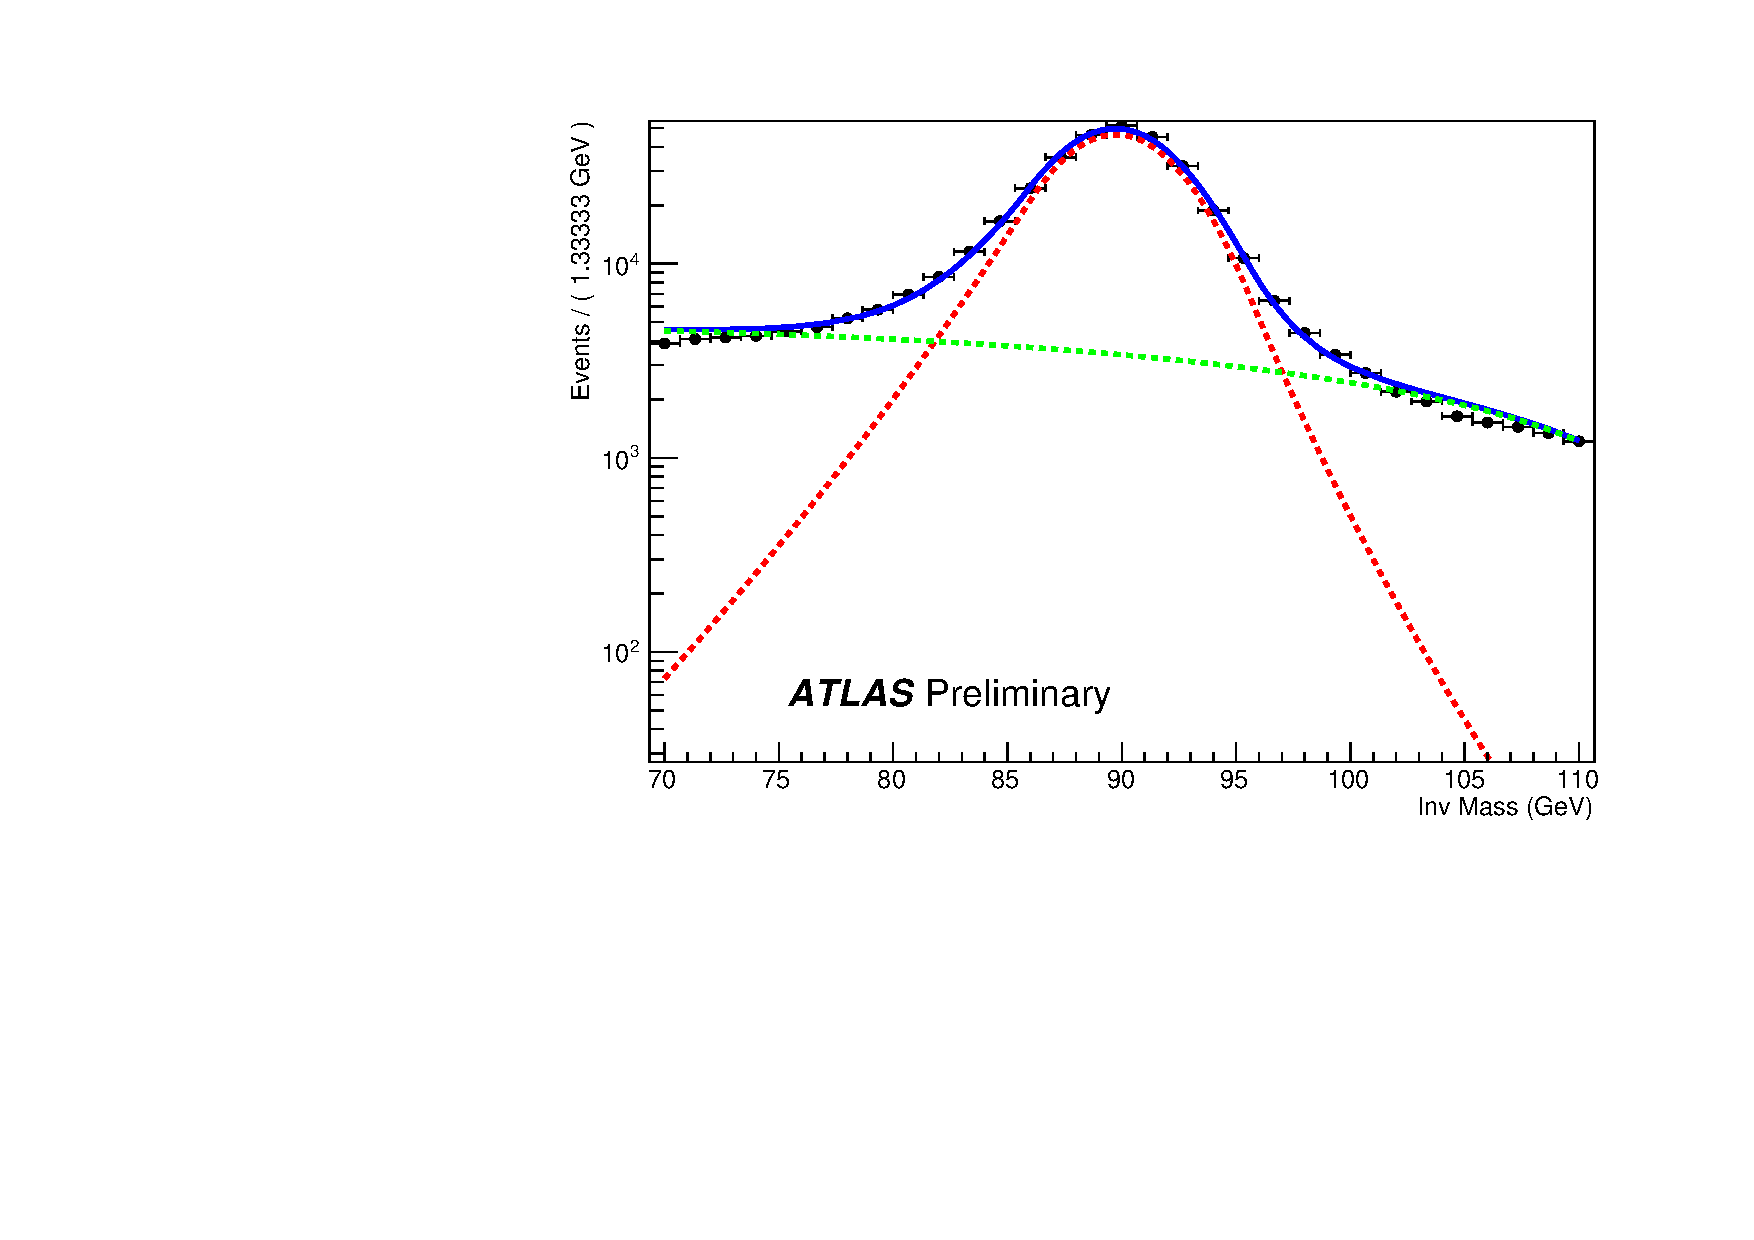
\includegraphics[scale=0.40]{d15_16_egam1_t_lmet_fit_h_m_eg_BB.pdf}
		\caption{Región BB}
	\end{subfigure}
	~
	\begin{subfigure}{0.5\textwidth}
		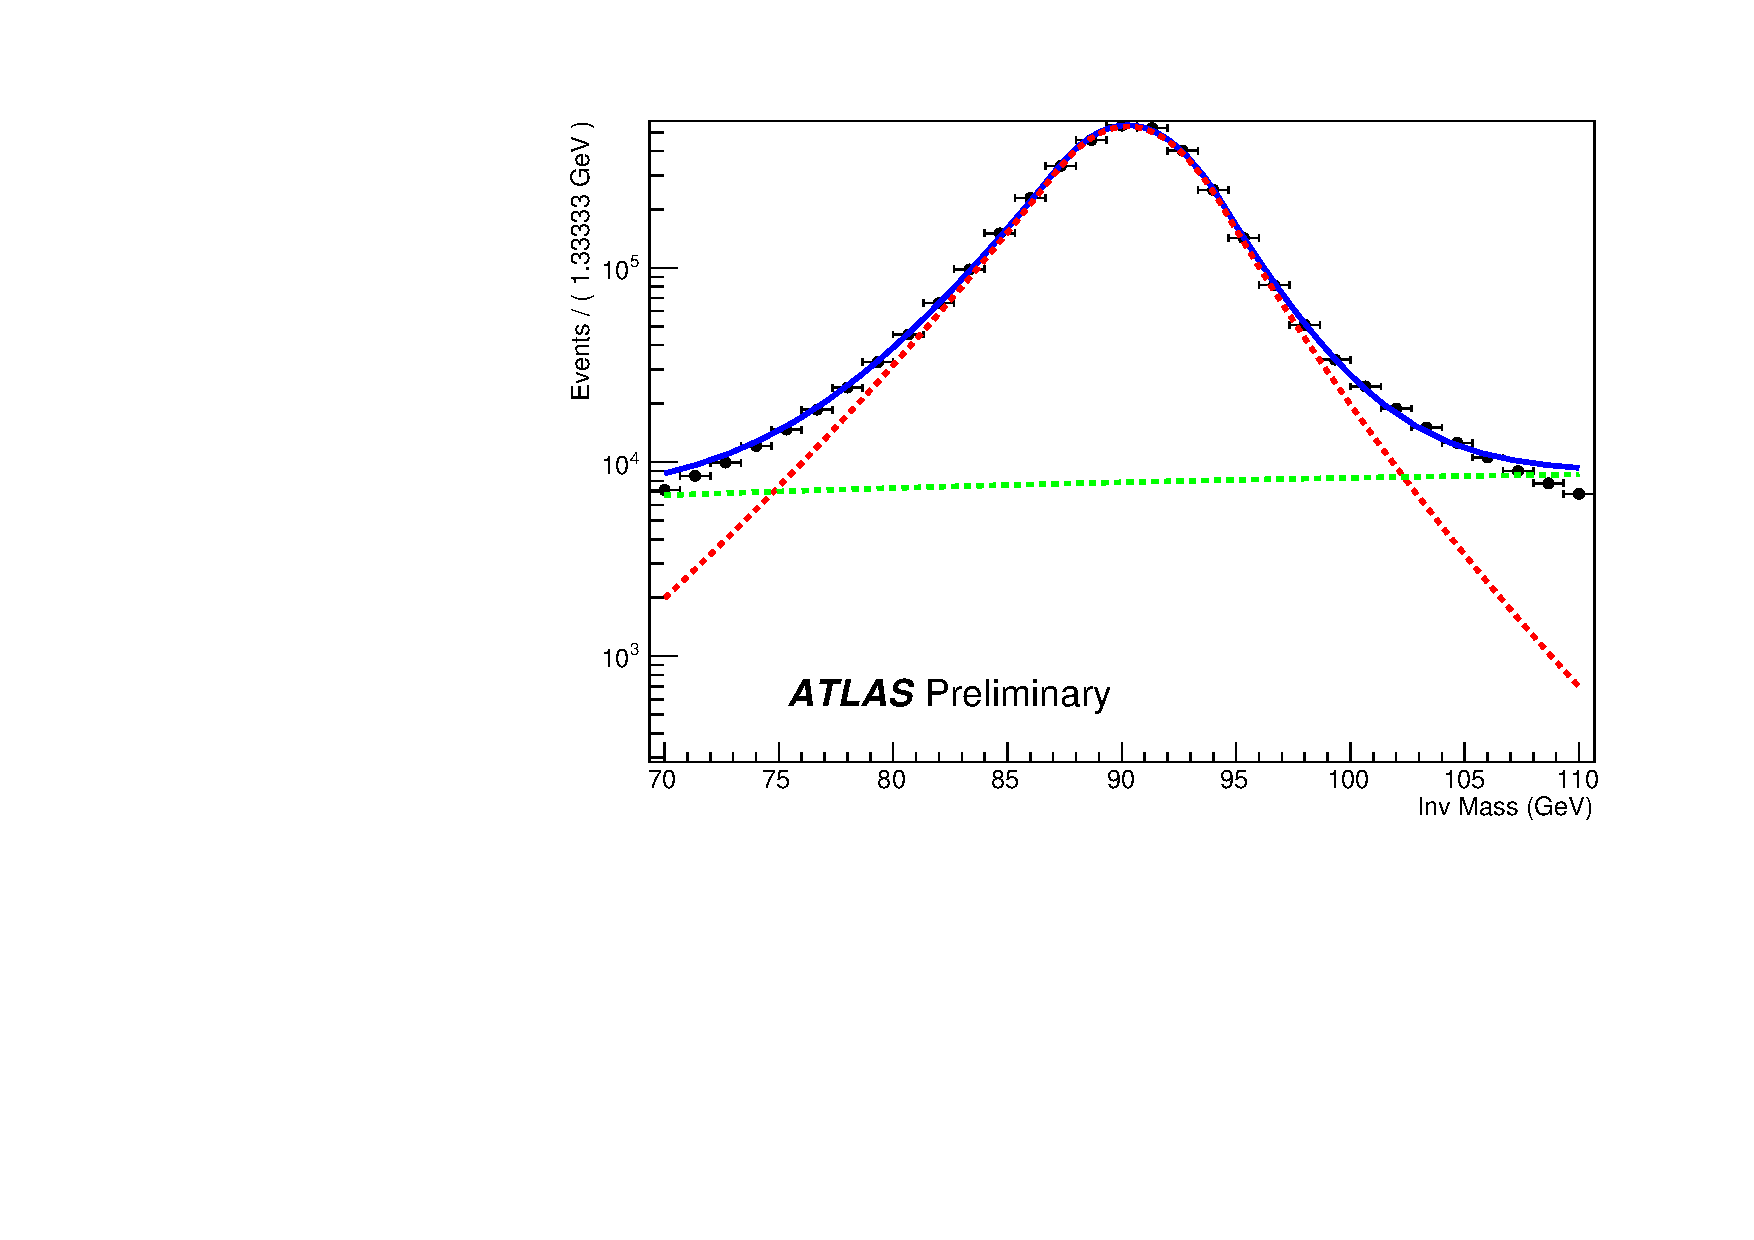
\includegraphics[scale=0.40]{d15_16_egam1_t_lmet_fit_h_m_ee_BE.pdf} 
		\caption{Región BE}
	\end{subfigure}
	~
	\begin{subfigure}{0.5\textwidth}
		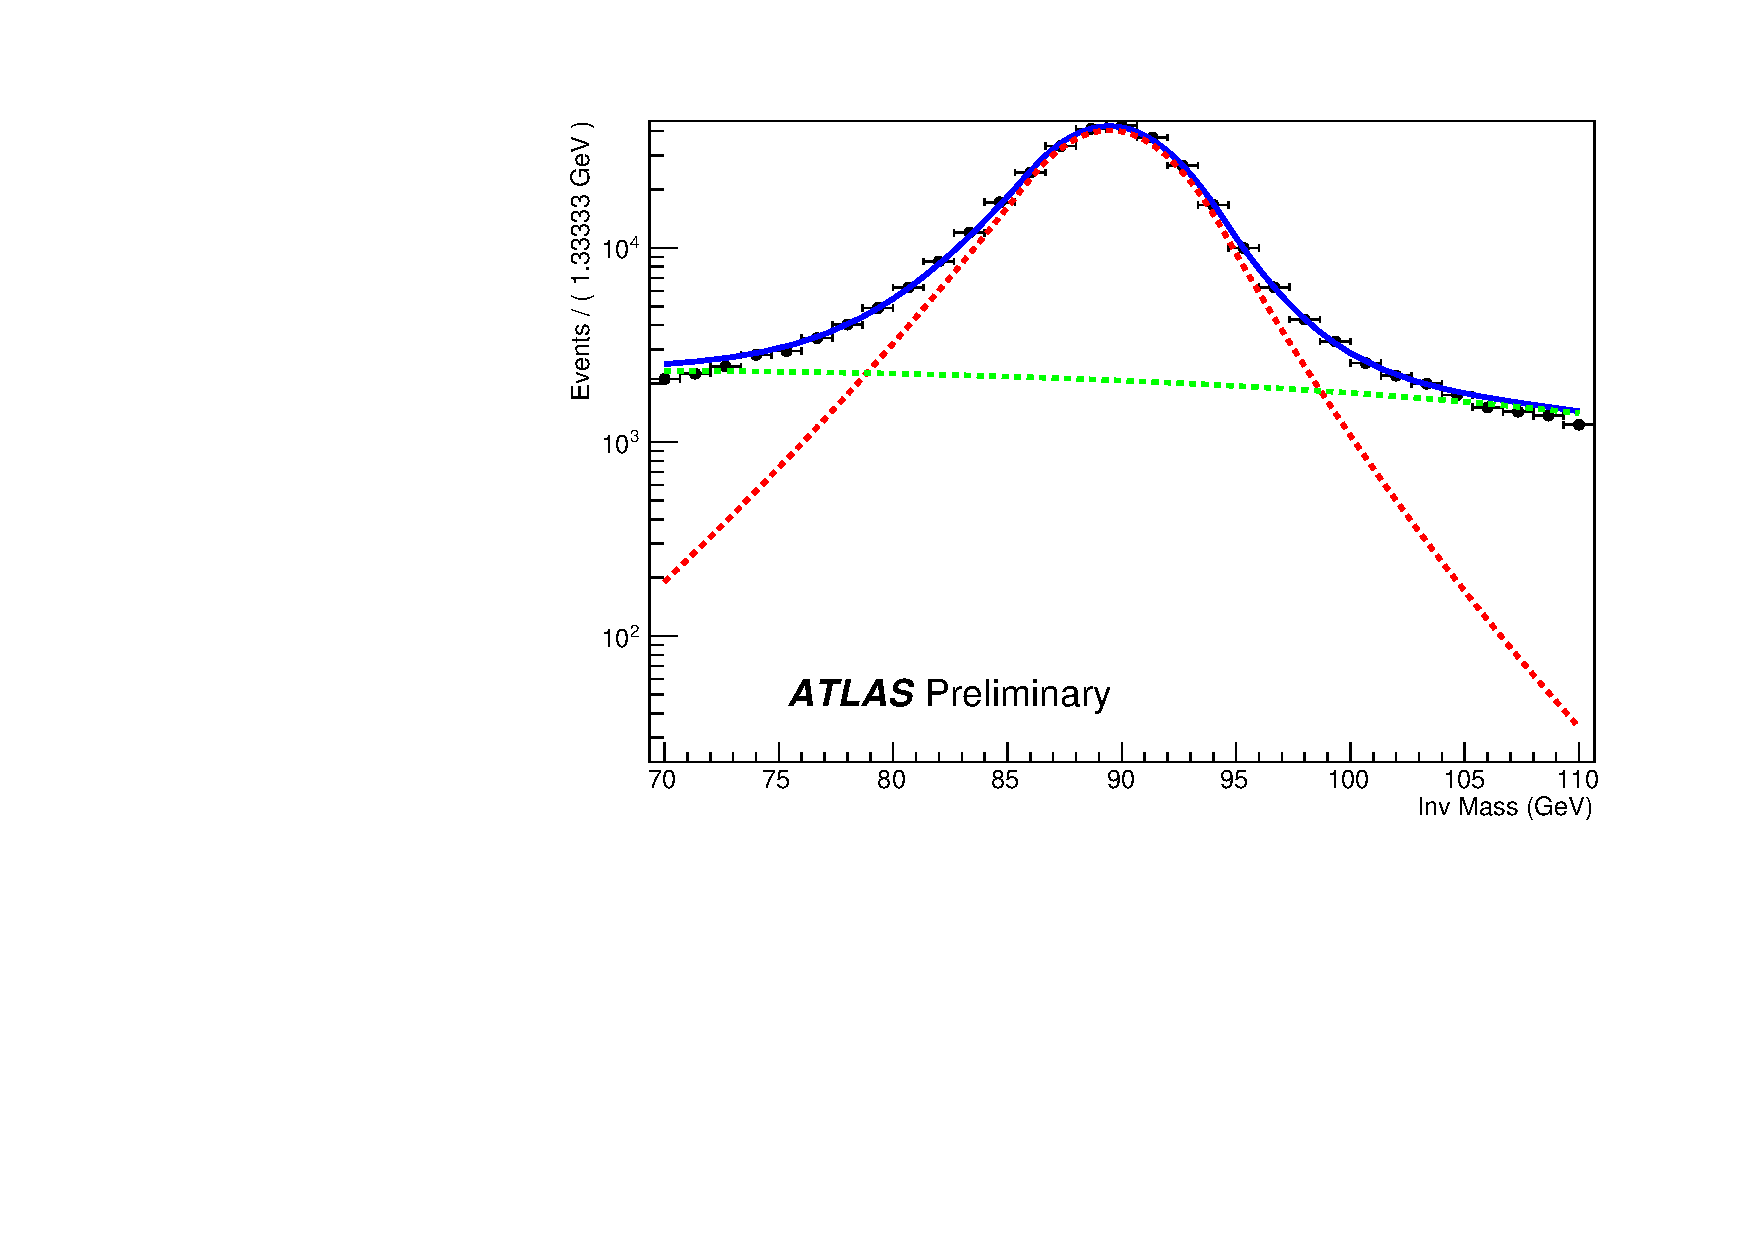
\includegraphics[scale=0.40]{d15_16_egam1_t_lmet_fit_h_m_eg_BE.pdf}
		\caption{Región BE}
	\end{subfigure}
	~
	\begin{subfigure}{0.5\textwidth}
		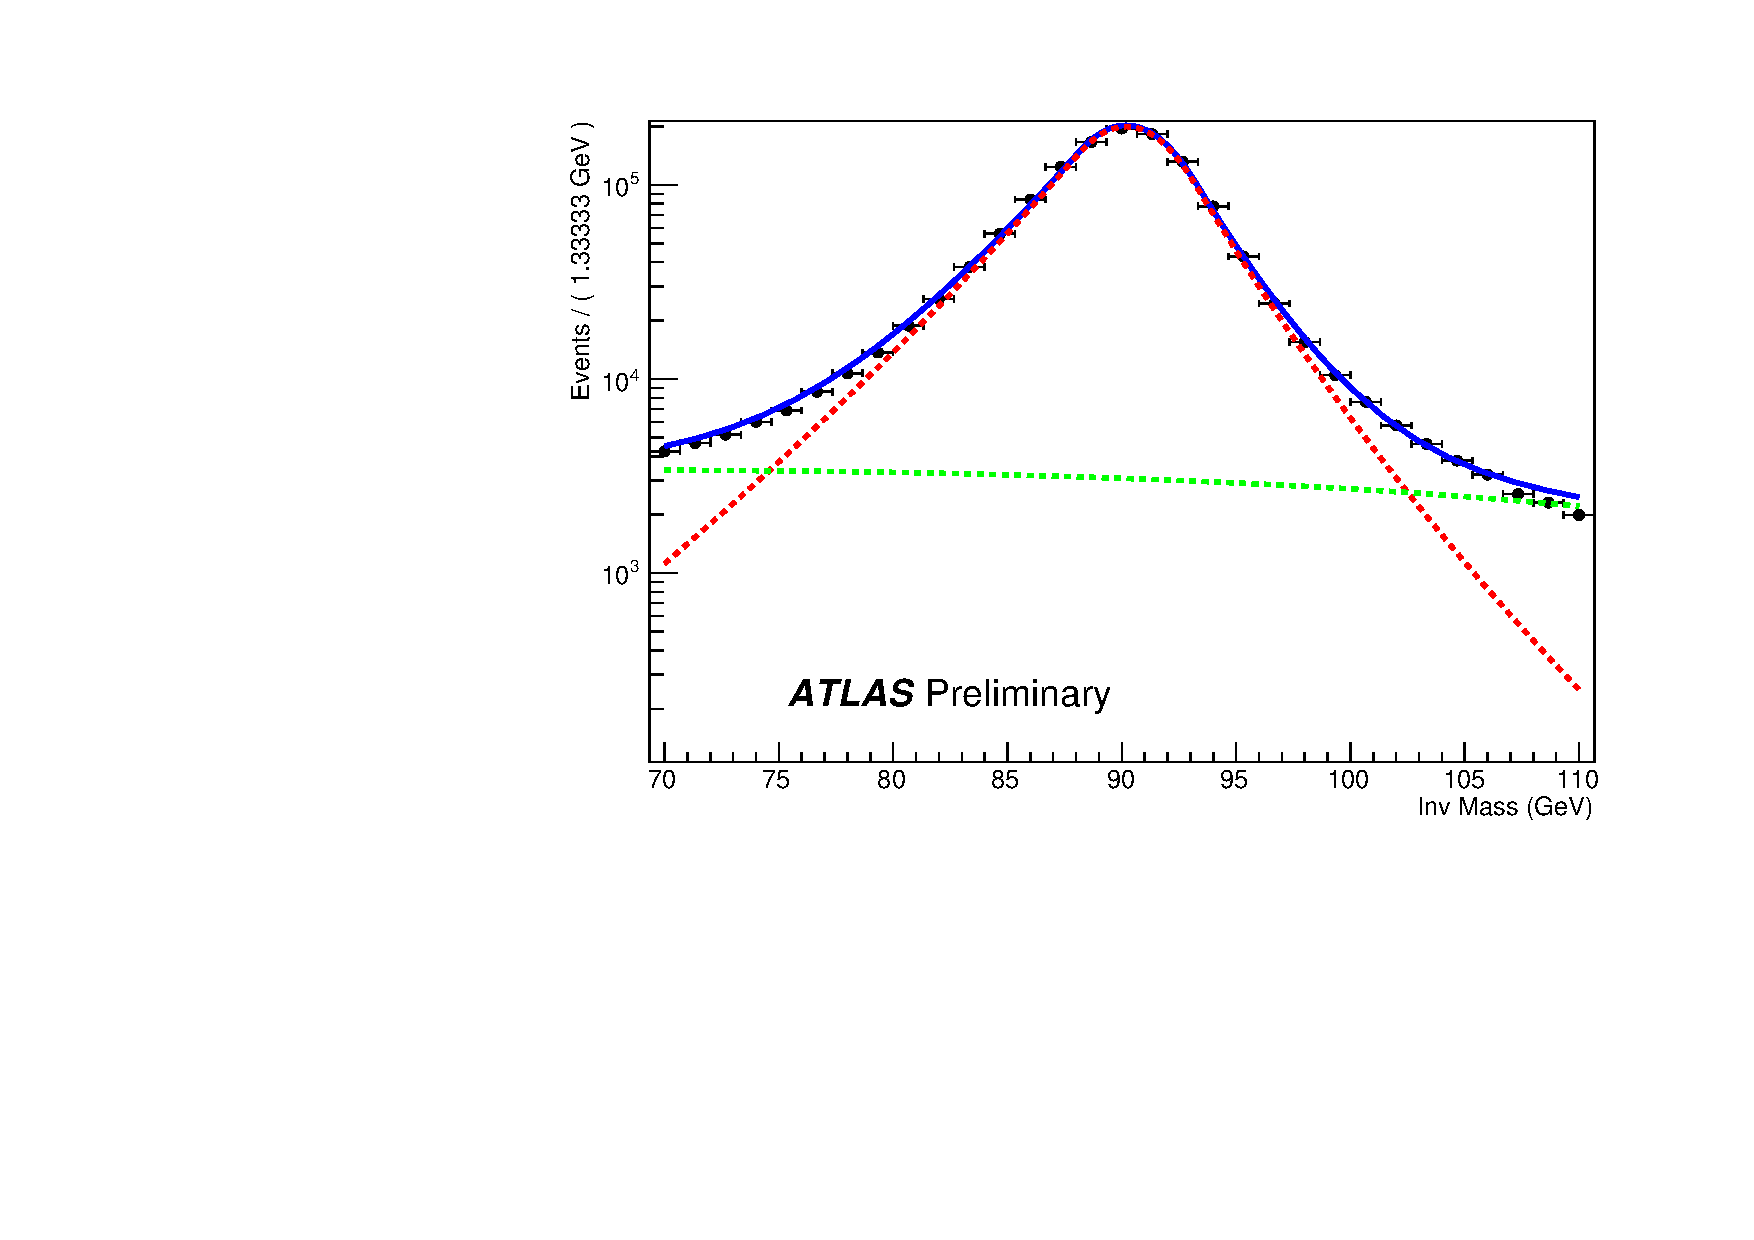
\includegraphics[scale=0.40]{d15_16_egam1_t_lmet_fit_h_m_ee_EE.pdf} 
		\caption{Región EE}
	\end{subfigure}
	~
	\begin{subfigure}{0.5\textwidth}
		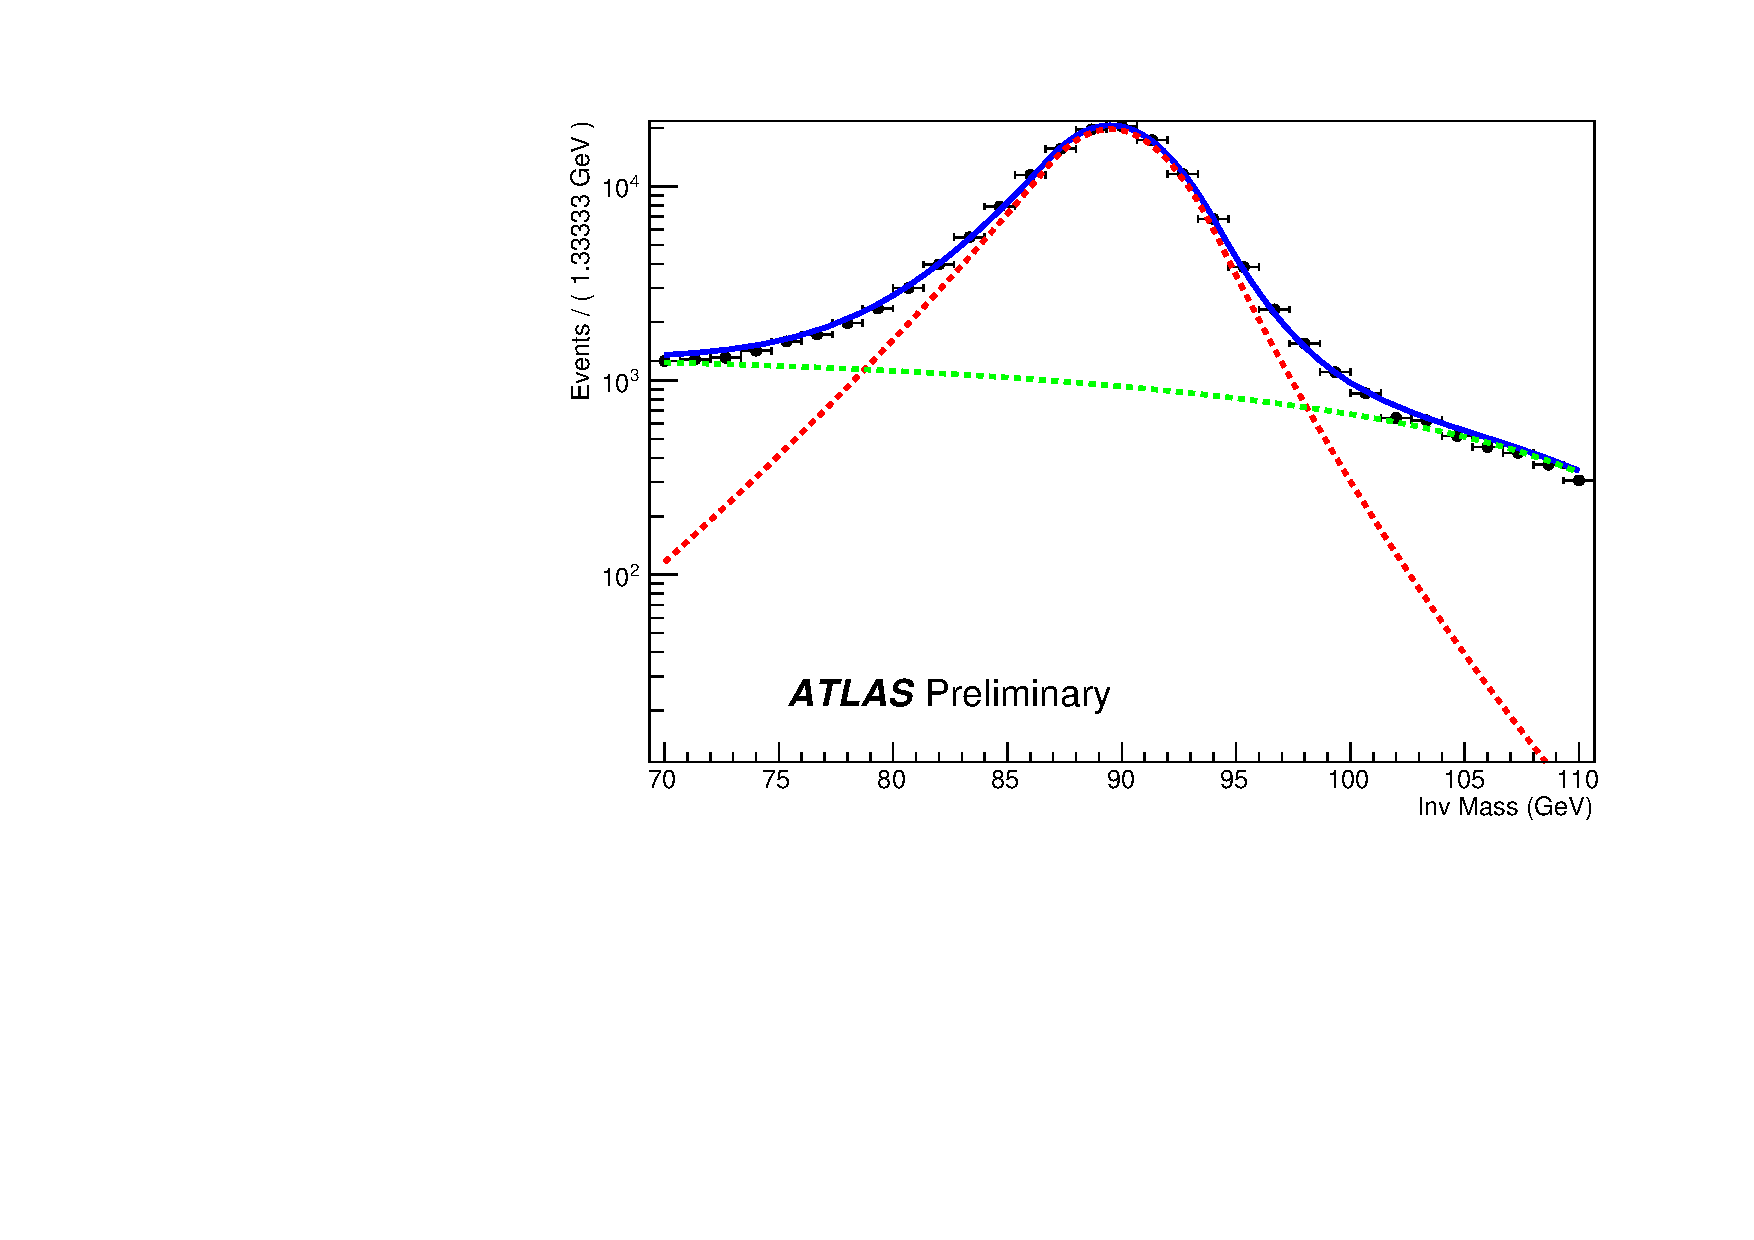
\includegraphics[scale=0.40]{d15_16_egam1_t_lmet_fit_h_m_eg_EE.pdf}
		\caption{Región EE}
	\end{subfigure}

	\caption{Ajuste de la masa invariante de los pares $ee$ (izquierda) y $e\gamma$ (derecha), para cada región de reconstrucción y para electrones \textit{tight}. La curva roja corresponde a la DSCB, la verde al polinomio de grado 2 y la azul a la combinación resultante de ambas.}
\label{fits_invmass_tight}
\end{figure}




\section{Resultados y estimación del fondo en regiones validación} \label{sec:resultados}


Los resultados obtenidos para el factor en bines de $\eta$ y $p_{T}$ para electrones \textit{medium} y \textit{tight} se muestran en la Tablas \ref{ta:fftable_medium} y \ref{ta:fftable_tight}, incluyendo por separada las incertezas estadísticas y sistemáticas del método. Se puede apreciar que este factor crece con $|\eta|$, dado que está relacionado con el incremento en el material del detector atravesado por los electrones y el incremento en la tasa de reconstrucción de fotones convertidos con una sola traza \cite{Alonso:2147473}.


\begin{table}	
\centering
\caption{Tabla con los factores de identificación errónea en bines de $\eta$ y $p_{T}$, con sus valores de incerteza estadística y sistemática, para electrones \textit{medium}.}
\begin{threeparttable}
\begin{tabular}{ l l c c c c c }

	\hline
	\hline

	\multirow{2}{*}{$|\eta|$} & \multirow{2}{*}{$p_{T}$[GeV]} & \multirow{2}{*}{Fake factor} & \multirow{2}{*}{Estadístico} & \multicolumn{3}{c}{Sistemáticos}  \\

	\cline{5-7}

	 		& & & 	& $w=1$ & Rango & Total \\


	\hline

	0 - 0.6 	& 75 - 90 	& 0.0149 & 0.0003 & 0.004	&  0.0004	&  0.004  \\

	0 - 0.6 	& 90 - 145 	& 0.0136 & 0.0004 & 0.004	&  0.0004	&  0.004  \\

	0 - 0.6 	& 145 - 300 & 0.0113 & 0.0008 & 0.003	&  0.0003	&  0.003  \\

	\hline

	0.6 - 1.37 	& 75 - 90 	& 0.0164 & 0.0003 & 0.004	&  0.0004	&  0.004  \\

	0.6 - 1.37 	& 90 - 145 	& 0.0157 & 0.0004 & 0.004	&  0.0003	&  0.004  \\

	0.6 - 1.37 	& 145 - 300 & 0.0116 & 0.0007 & 0.003	&  0.0003	&  0.003  \\

	\hline

	1.52 - 1.82 & 75 - 90 	& 0.034  & 0.001 & 0.005	&  0.0005	&  0.005 \\

	1.52 - 1.82 & 90 - 145 	& 0.030  & 0.001 & 0.005	&  0.001	&  0.005  \\

	1.52 - 1.82 & 145 - 300 & 0.023  & 0.002 & 0.003	&  0.0005	&  0.003  \\

	\hline

	1.82 - 2.37 & 75 - 90 	& 0.044		& 0.001 & 0.006	&  0.002	&  0.006  \\

	1.82 - 2.37 & 90 - 145	& 0.038		& 0.001 & 0.005	&  0.001	&  0.005  \\

	1.82 - 2.37 & 145 - 300 & 0.039		& 0.003 & 0.006	&  0.001	&  0.006  \\

	\hline
	\hline

\end{tabular}
\end{threeparttable}
\label{ta:fftable_medium}
\end{table}

\begin{table}	
\centering
\caption{Tabla con los factores de identificación errónea en bines de $\eta$ y $p_{T}$, con sus valores de incerteza estadística y sistemática, para electrones \textit{tight}.}
\begin{threeparttable}
\begin{tabular}{ l l c c c c c }

	\hline
	\hline

	\multirow{2}{*}{$|\eta|$} & \multirow{2}{*}{$p_{T}$[GeV]} & \multirow{2}{*}{Fake factor} & \multirow{2}{*}{Estadístico} & \multicolumn{3}{c}{Sistemáticos} \\
	
	\cline{5-7}

	 & & & & $w=1$ & Rango & Total \\

	\hline

	0 - 0.6 	& 75 - 90 	& 0.0155 & 0.0004 & 0.004	&  0.001	&  0.004  \\

	0 - 0.6 	& 90 - 145 	& 0.0141 & 0.0004 & 0.004	&  0.002	&  0.004  \\

	0 - 0.6 	& 145 - 300 & 0.0116 & 0.0008 & 0.002	&  0.001	&  0.003  \\

	\hline

	0.6 - 1.37 	& 75 - 90 	& 0.0173 & 0.0004 & 0.004	&  0.002	&  0.004  \\

	0.6 - 1.37 	& 90 - 145 	& 0.0161 & 0.0004 & 0.004	&  0.002	&  0.004  \\

	0.6 - 1.37 	& 145 - 300 & 0.0121 & 0.0008 & 0.003	&  0.002	&  0.003  \\

	\hline

	1.52 - 1.82 & 75 - 90 	& 0.036  & 0.001 & 0.005	&  0.002	&  0.005 \\

	1.52 - 1.82 & 90 - 145 	& 0.033  & 0.001 & 0.004	&  0.003	&  0.005  \\

	1.52 - 1.82 & 145 - 300 & 0.022  & 0.002 & 0.003	&  0.001	&  0.003  \\

	\hline

	1.82 - 2.37 & 75 - 90 	& 0.046		& 0.001 & 0.007	&  0.002	&  0.007  \\

	1.82 - 2.37 & 90 - 145	& 0.039		& 0.001 & 0.006	&  0.003	&  0.007  \\

	1.82 - 2.37 & 145 - 300 & 0.041		& 0.003 & 0.006	&  0.002	&  0.006  \\

	\hline
	\hline

\end{tabular}
\end{threeparttable}
\label{ta:fftable_tight}
\end{table}

% \begin{table}	
% \centering
% \begin{threeparttable}
% \caption{Tabla con los factores de identificación errónea en bines de $\eta$ y $p_{T}$, con sus valores de incerteza estadística y sistemática.}
% \begin{tabular}{ l l c c c }

% 	\hline
% 	\hline

% 	$|\eta|$ & $p_{T}$[GeV] & Fake factor & Estadísticos & Sistemáticos \\

% 	\hline

% 	0 - 0.6 & 75 - 90 & 0.0168 & 0.0003 & -		 \\

% 	0 - 0.6 & 90 - 145 & 0.0158 & 0.0004 & - 	 \\

% 	0 - 0.6 & 145 - 300 & 0.0142 & 0.0007 & -  	 \\

% 	\hline

% 	0.6 - 1.37 & 75 - 90 & 0.0186 & 0.0003 & -	 \\

% 	0.6 - 1.37 & 90 - 145 & 0.0183 & 0.0004 & -	 \\

% 	0.6 - 1.37 & 145 - 300 & 0.0141 & 0.0007 & -   \\

% 	\hline

% 	1.52 - 1.82 & 75 - 90 & 0.0354  & 0.0009 &  \\

% 	1.52 - 1.82 & 90 - 145 & 0.033  & 0.001 & \\

% 	1.52 - 1.82 & 145 - 300 & 0.026  & 0.002 & \\

% 	\hline

% 	1.82 - 2.37 & 75 - 90 & 0.045  & 0.001 &  \\

% 	1.82 - 2.37 & 90 - 145 & 0.040  & 0.001 &  \\

% 	1.82 - 2.37 & 145 - 300 & 0.038  & 0.002 & \\

% 	\hline
% 	\hline

% \end{tabular}
% \label{ta:fftable}
% \end{threeparttable}
% \end{table}

Observando los resultados expuestos en las distintas tablas, definimos la implementación de una selección \textit{medium} de los electrones ya que los valores de pureza (expresado en los valores de los pesos $w$) e incertezas sistemáticas son equivalentes a la selección \textit{tight}, pero con la ventaja de una probable mayor estadística de eventos para estimar el fondo en las distintas regiones de control y validación.


Con el objetivo de validar los resultados obtenidos, se realizo una búsqueda de una nueva región de validación donde el fondo predominante sea el de eventos con electrones erróneamente reconstruidos. Los criterios para determinar la VR se pueden observar en la Tabla \ref{ta:vr_crit}. Estos criterios seleccionan de forma predominante eventos $W(e\nu)$ + jets, donde un $W$ con alta energía cinética, decae en un neutrino (asociado con una alta $\met$) y electrón de alto $p_{T}$ (identificado como fotón), son colineales entre sí ($\Delta\phi<0.4$). La contribución de cada fondo al número de eventos en esta región se puede observar en la Tabla \ref{ta:vr_events}, en donde se puede observar que para esta región el fondo proveniente de electrones mal reconstruidos como fotones es el que predomina ($\sim63\%$) y se observa comparativamente un excelente acuerdo entre los datos esperados y obtenidos. Las distribuciones para $\Delta \phi$ y $\met$ se observan en las Figuras \ref{VRE_dphi} y \ref{VRE_met_et}, donde se observa un excelente acuerdo entre las los resultados esperados y los datos obtenidos.

Los resultados mostrados permiten entonces validar el método y sus predicciones, y poder ser así utilizados para predecir la cantidad de eventos esperados en las distintas regiones de señal.

\begin{table}
\centering
\caption{Criterios de selección para la región de validación \cite{drfran}.}
  \begin{tabular}{l|r}
  \hline
  \hline
  & VRE \\
  \hline
  $N_{\mathrm{fotones}}$                  &       $\ge1$  \\
  $\pt^{\text{leading}\: \gamma} >$         &    $145\egev$  \\
  $N_{\mathrm{leptones}}$                  &           -   \\
  $N_{\mathrm{jets}}$                     &       $\ge1$  \\
  $N_{b-\mathrm{jets}}$                   &       $\ge1$  \\
  $\Delta\phi(\text{jet}, \met)$          &       $>0.4$  \\
  $\Delta\phi(\gamma, \met)$                &       $<0.4$  \\
  ${\met}$                                &   $>200\egev$  \\
  $m_{\text{eff}}$                               &  $[500, 2000]\egev$  \\
  \hline
  \hline
\end{tabular}
\label{ta:vr_crit}
\end{table}

\begin{table}
\centering
\caption{Contribución de cada fondo a la región de validación. Las incertezas mostradas son solo sistemáticas \cite{drfran}.}
\begin{tabular}{lr}
\hline
 & $e\to\gamma$ falsos VR \\
\hline
Eventos observados & 94 \\
\hline
Eventos esperados por el SM & $92.18 \pm 12.58$ \\
\hline
$\gamma$ + jets & $1.46 \pm 0.16$ \\
$W\gamma$ & $13.73 \pm 1.26$ \\
$Z\gamma$ & $0.87 \pm 0.05$ \\
$\ttbar\gamma$ & $4.91 \pm 0.70$ \\
$e\rightarrow\gamma$ falsos & $58.43 \pm 12.49$ \\
$\text{jets}\rightarrow\gamma$ falsos & $12.73 \pm 2.14$ \\
$\gamma\gamma / W\gamma\gamma / Z\gamma\gamma$ & $0.05 \pm 0.00$ \\
\hline
\end{tabular}
\label{ta:vr_events}
\end{table}


\begin{figure}
\centering
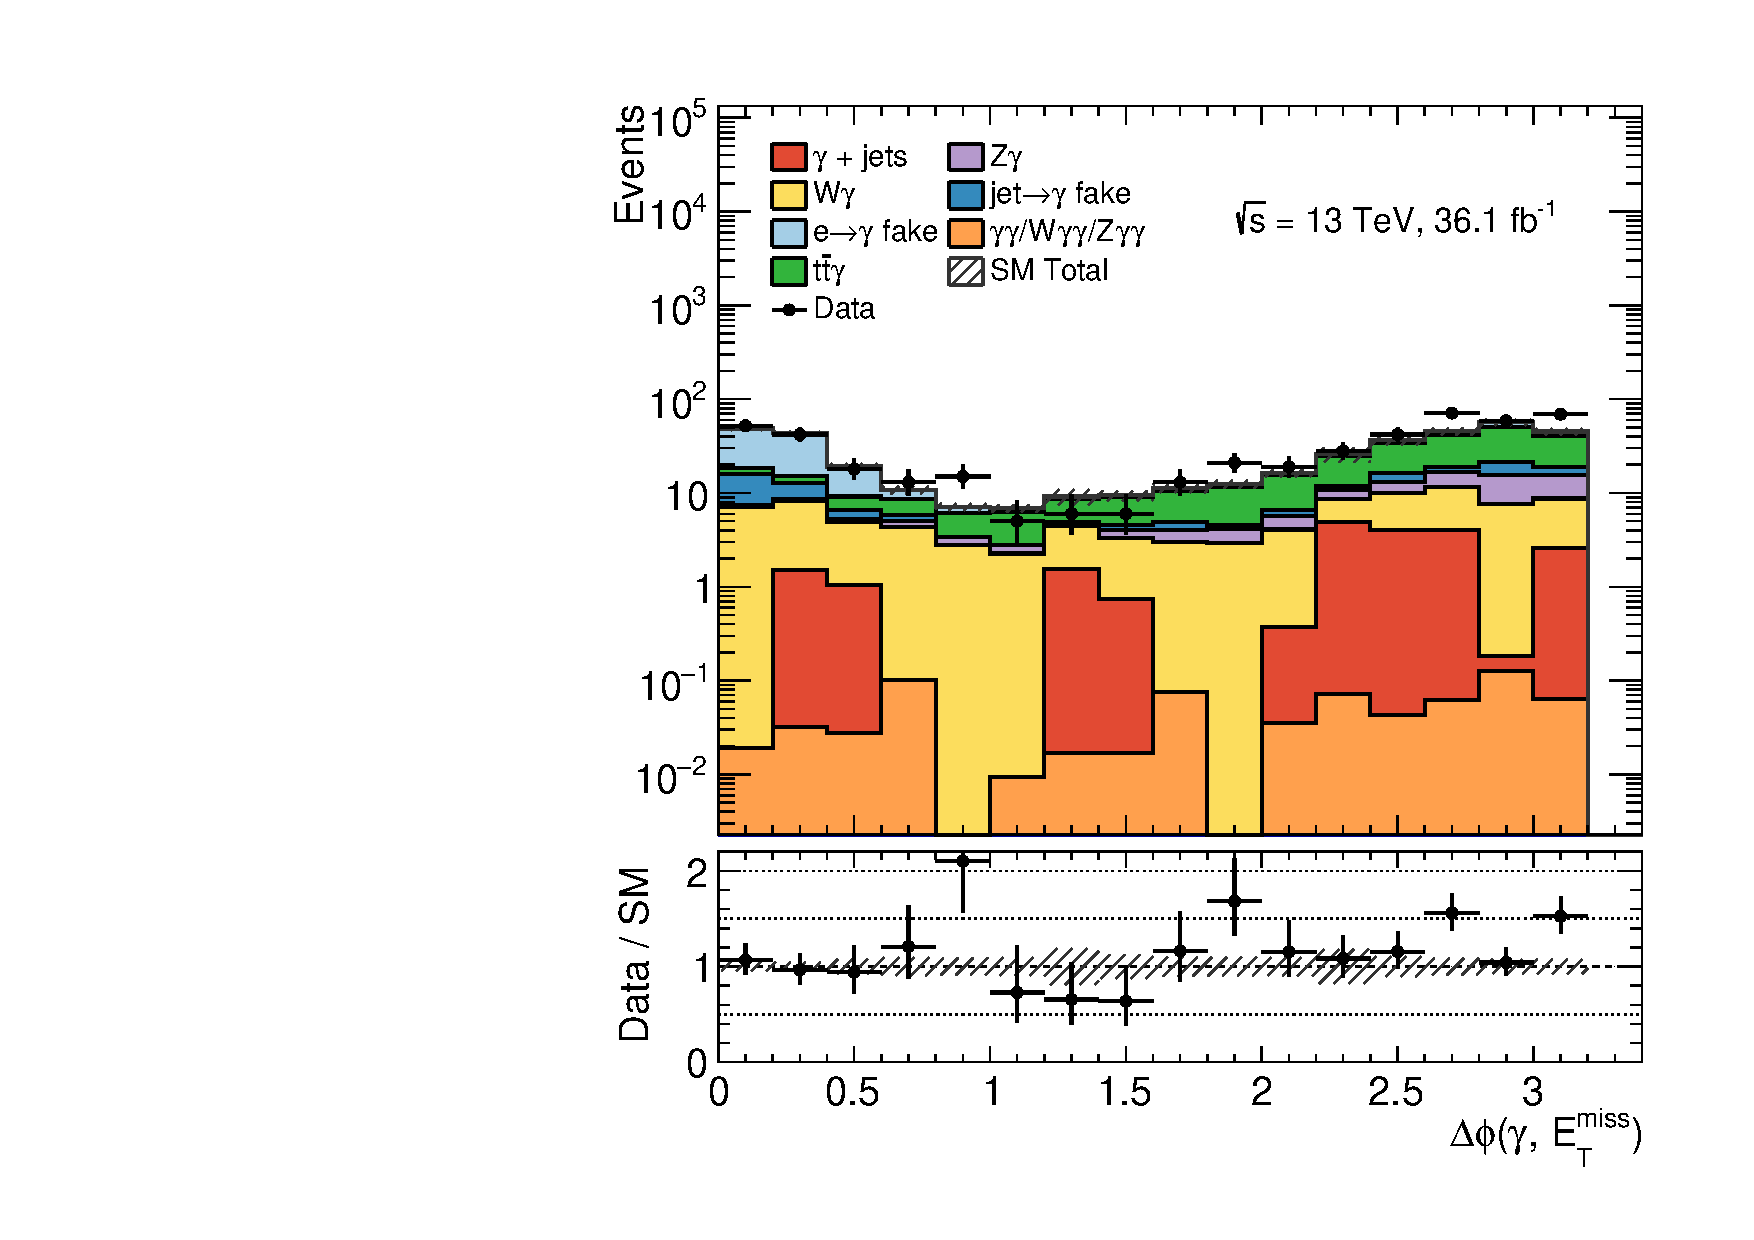
\includegraphics[width=0.50\textwidth]{can_VRE_dphi_gammet_afterFit.pdf}
\caption{Distribución de $\Delta \phi$ para una región de validación. La variable mostrada se deja libre en el gráfico, mientras el resto de la variables se mantienen con los cortes propuestos en la VRE. Las incertezas mostradas son solo estadísticas \cite{drfran}.}
\label{VRE_dphi}
\end{figure}

\begin{figure}
\centering
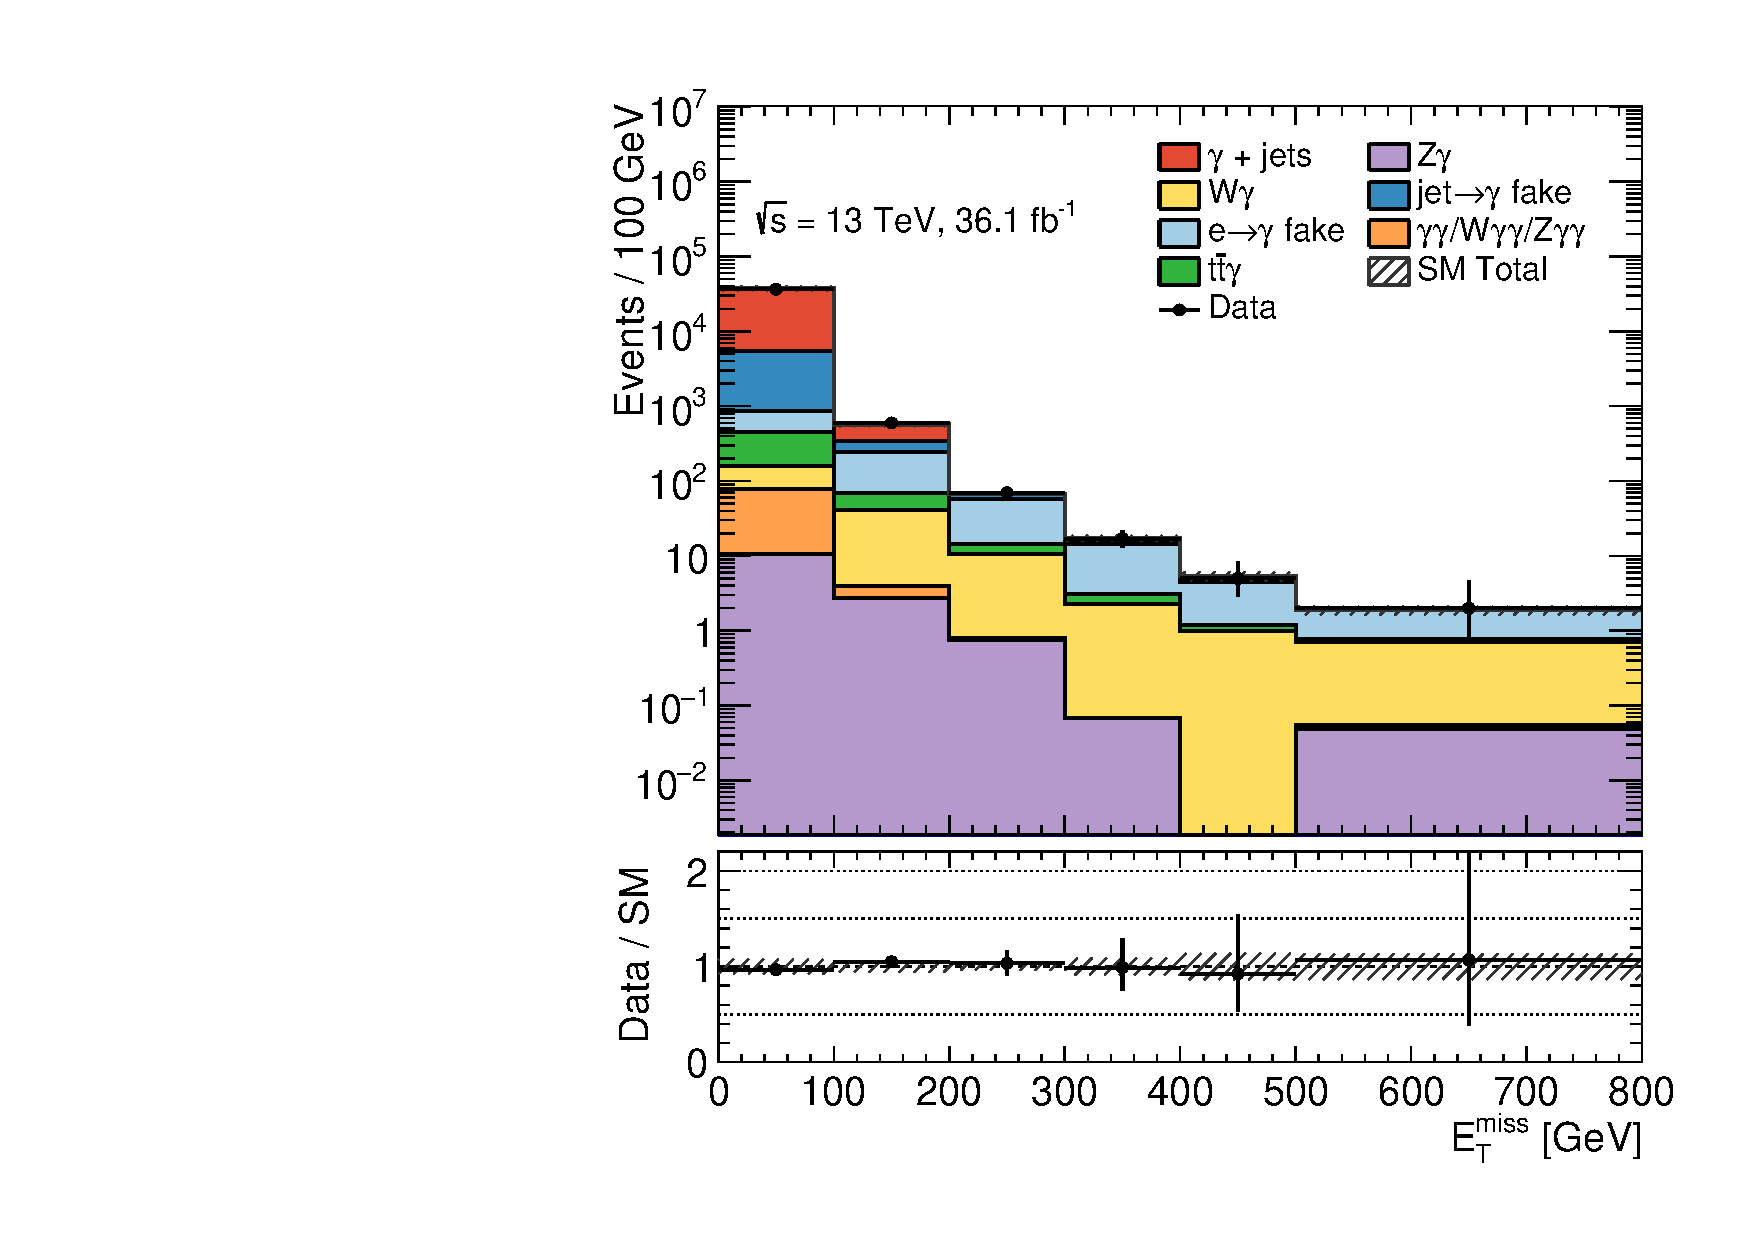
\includegraphics[width=0.50\textwidth]{can_VRE_met_et_afterFit.pdf}
\caption{Distribución de $\met$ para una región de validación. La variable mostrada se deja libre en el gráfico, mientras el resto de la variables se mantienen con los cortes propuestos en la VRE. Las incertezas mostradas son solo estadísticas \cite{drfran}.}
\label{VRE_met_et}
\end{figure}



\clearpage